\documentclass[12pt]{article}
\usepackage[margin=1in]{geometry}

% TODO: Create the following new visualizations to enhance research presentation:
% 1. Multi-factor Analysis Chart: Showing interaction between model type, fusion method, and dataset
% 2. Ablation Study Visualization: Demonstrating impact of removing different components
% 3. Error Analysis Heat Map: Showing which emotion pairs are most frequently confused
% 4. Performance vs Complexity Graph: Plotting accuracy against model size/inference time
% 5. Learning Curve Comparison: Showing how different models learn over training epochs
% 6. Feature-Fusion Performance Matrix: A heatmap showing how different audio feature and fusion 
%    strategy combinations perform

% The preceding line only needs to identify funding in the first footnote. If that is unnecessary, please comment on it.
\usepackage{float}
\usepackage[table]{xcolor}
\usepackage{cite}
\usepackage{subcaption}
\usepackage{multirow}
\usepackage{graphicx}
\usepackage{amsmath,amssymb,amsfonts}
\usepackage{algorithmic}
\usepackage{graphicx}
\usepackage{textcomp}
\usepackage{xcolor}
\usepackage{multirow}
\usepackage{setspace}
\usepackage{tabularx}
\usepackage{url}
\usepackage{tabularray}
\usepackage{makecell}
\usepackage{placeins}
\usepackage{comment}
\usepackage{verbatim}
\usepackage{rotating}
\usepackage{changepage}
\renewcommand{\cellalign}{cl}

\usepackage{booktabs, multirow} % for borders and merged ranges
\usepackage{soul}% for underlines
\usepackage[table]{xcolor} % for cell colors
\usepackage{threeparttable} % for wide tables

\usepackage{pdflscape}  % For landscape environment
\usepackage{adjustbox}  % For adjustbox environment

\def\BibTeX{{\rm B\kern-.05em{\sc i\kern-.025em b}\kern-.08em
    T\kern-.1667em\lower.7ex\hbox{E}\kern-.125emX}}
    
    
    \newcommand*{\affaddr}[1]{#1} % No op here. Customize it for different styles.
\newcommand*{\affmark}[1][*]{\textsuperscript{#1}}
\newcommand*{\email}[1]{\textit{#1}}
    
\begin{document}
\begin{center}
\Large
\thispagestyle{empty}

\textbf{Two-Stage Emotion Detection from Multimodal Data}\\
\vspace{0.1in}
\large
\text{A Project Report}\\
\vspace{2in}

\text{Presented to}\\
\text{The Faculty of the Department of Computer Science}\\
\text{San Jose State University}\\

\vspace{1in}

\text{In Partial Fulfillment}\\
\text{of the Requirements for the Degree of}\\
\text{Master of Science}\\

\vspace{1in}

\text{By}\\
\text{Xiangyi Li}\\
\text{Spring 2024}\\

\end{center}

\title{}
\newpage
\thispagestyle{empty}
\begin{center}
\Large
\text{The Designated Project Committee Approves the Project Titled}\\
\vspace{0.1in}
\Large
\text{Two-Stage Emotion Detection from Multimodal Data}\\
\vspace{0.5in}
\text{by}\\
\vspace{0.1in}
\text{Xiangyi Li}\\
\vspace{1.5in}
\Large
\text{APPROVED FOR THE DEPARTMENT OF COMPUTER SCIENCE} \\
\vspace{0.1in}
\text{SAN JOSÉ STATE UNIVERSITY} \\
\vspace{0.1in}
\text{Spring 2024}\\
\vspace{1.5in}
\Large
\begin{tabular}{lcl}
Prof. Faranak Abri & \hspace{1cm} & Department of Computer Science \\
Prof. Fabio Di Troia & \hspace{1cm} & Department of Computer Science \\
Ms. Shuyi Wang & \hspace{1cm} & International Monetary Fund
\end{tabular}
 

\end{center}
\newpage

\pagenumbering{roman}
%\linespread{1.5} 

\doublespacing
\section{Introduction}
\label{sec:intro}
Emotion recognition plays a fundamental role in human communication, allowing us to understand others' feelings, intentions, and needs. As artificial intelligence systems become increasingly integrated into our daily lives, the ability for machines to recognize and respond appropriately to human emotions has become crucial for meaningful human-computer interaction. This capability, often referred to as affective computing, has applications ranging from healthcare and education to entertainment and customer service.

The structure of this report is as follows: Section \ref{sec:related} reviews relevant literature on emotion recognition approaches. Section \ref{sec:methodology} describes our methodology, including model architectures and the two-stage mapping process. Section \ref{sec:experimental_setup} details the experimental setup, covering dataset preparation, preprocessing techniques, and evaluation metrics. Section \ref{sec:results} presents our findings, focusing on the performance of AVD prediction and subsequent categorical mapping. Section \ref{sec:discussion} discusses the implications of our results and compares the two-stage approach with direct classification. Finally, Section \ref{sec:conclusion} concludes the report and suggests directions for future research.\section{Related Work}
\label{sec:related_work}

\textbf{Hybrid / fine-grained fusion} combines both.  Tensor Fusion
Networks \cite{zadeh2018multimodal_tfn}, Memory Fusion Networks
\cite{zadeh2018mfn}, capsule-based interaction
\cite{wang2019words} and cross-modal transformers
\cite{tsai2019mult} explicitly model inter-modal dynamics and achieve
the best overall results (e.g., 89 \% accuracy on CMU-MOSEI
\cite{mittal2020m3er}).

\subsection{Benchmark Datasets}
\textbf{IEMOCAP} \cite{busso2008iemocap} remains the de-facto benchmark
($\sim$10 k utterances, 9 emotions, audio+video+transcripts).  
\textbf{CMU-MOSI} \cite{zadeh2016mosi} and
\textbf{CMU-MOSEI} \cite{zadeh2018multimodal} provide large
"in-the-wild'' video reviews with sentiment and six-emotion labels.
\textbf{MELD} \cite{poria2018meld} introduces multi-party dialogue
context; \textbf{RAVDESS} \cite{livingstone2018ravdess} supplies
balanced acted speech.  Each poses distinct challenges in spontaneity,
noise and class imbalance, motivating the use of unweighted metrics
(UAR, UF1) alongside accuracy and weighted F1.

With deep learning, Convolutional Neural Networks (CNNs) have been applied directly to spectrograms, treating them as images and learning relevant patterns automatically~\cite{mao2014learning}. This approach eliminates the need for handcrafted feature engineering while often improving performance.

Hybrid fusion combines aspects of both early and late fusion, often using attention mechanisms to dynamically weight different modalities based on their relevance~\cite{zadeh2018memory}. These approaches have shown promising results by adapting to varying reliability of modalities across different inputs.\section{Methodology}
\label{sec:methodology}
Our approach to emotion detection employs a two-stage architecture that first predicts dimensional emotion values (Arousal, Valence, Dominance) from textual and audio modalities separately, then maps these dimensional representations to discrete emotion categories. This section provides a comprehensive overview of our methodology, including detailed descriptions of model architectures, audio feature extraction techniques, training procedures, and the mapping process between dimensional and categorical representations.

\subsection{System Architecture Overview}
Figure~\ref{fig:system_architecture} illustrates the high-level architecture of our two-stage emotion detection system. The first stage consists of separate processing pipelines for textual and audio data, each optimized for the specific characteristics of its modality and trained to predict continuous AVD values. The second stage implements a mapping function that translates the predicted dimensional values into discrete emotion categories, leveraging the structured nature of the dimensional emotion space.

\begin{figure}[h]
    \centering
    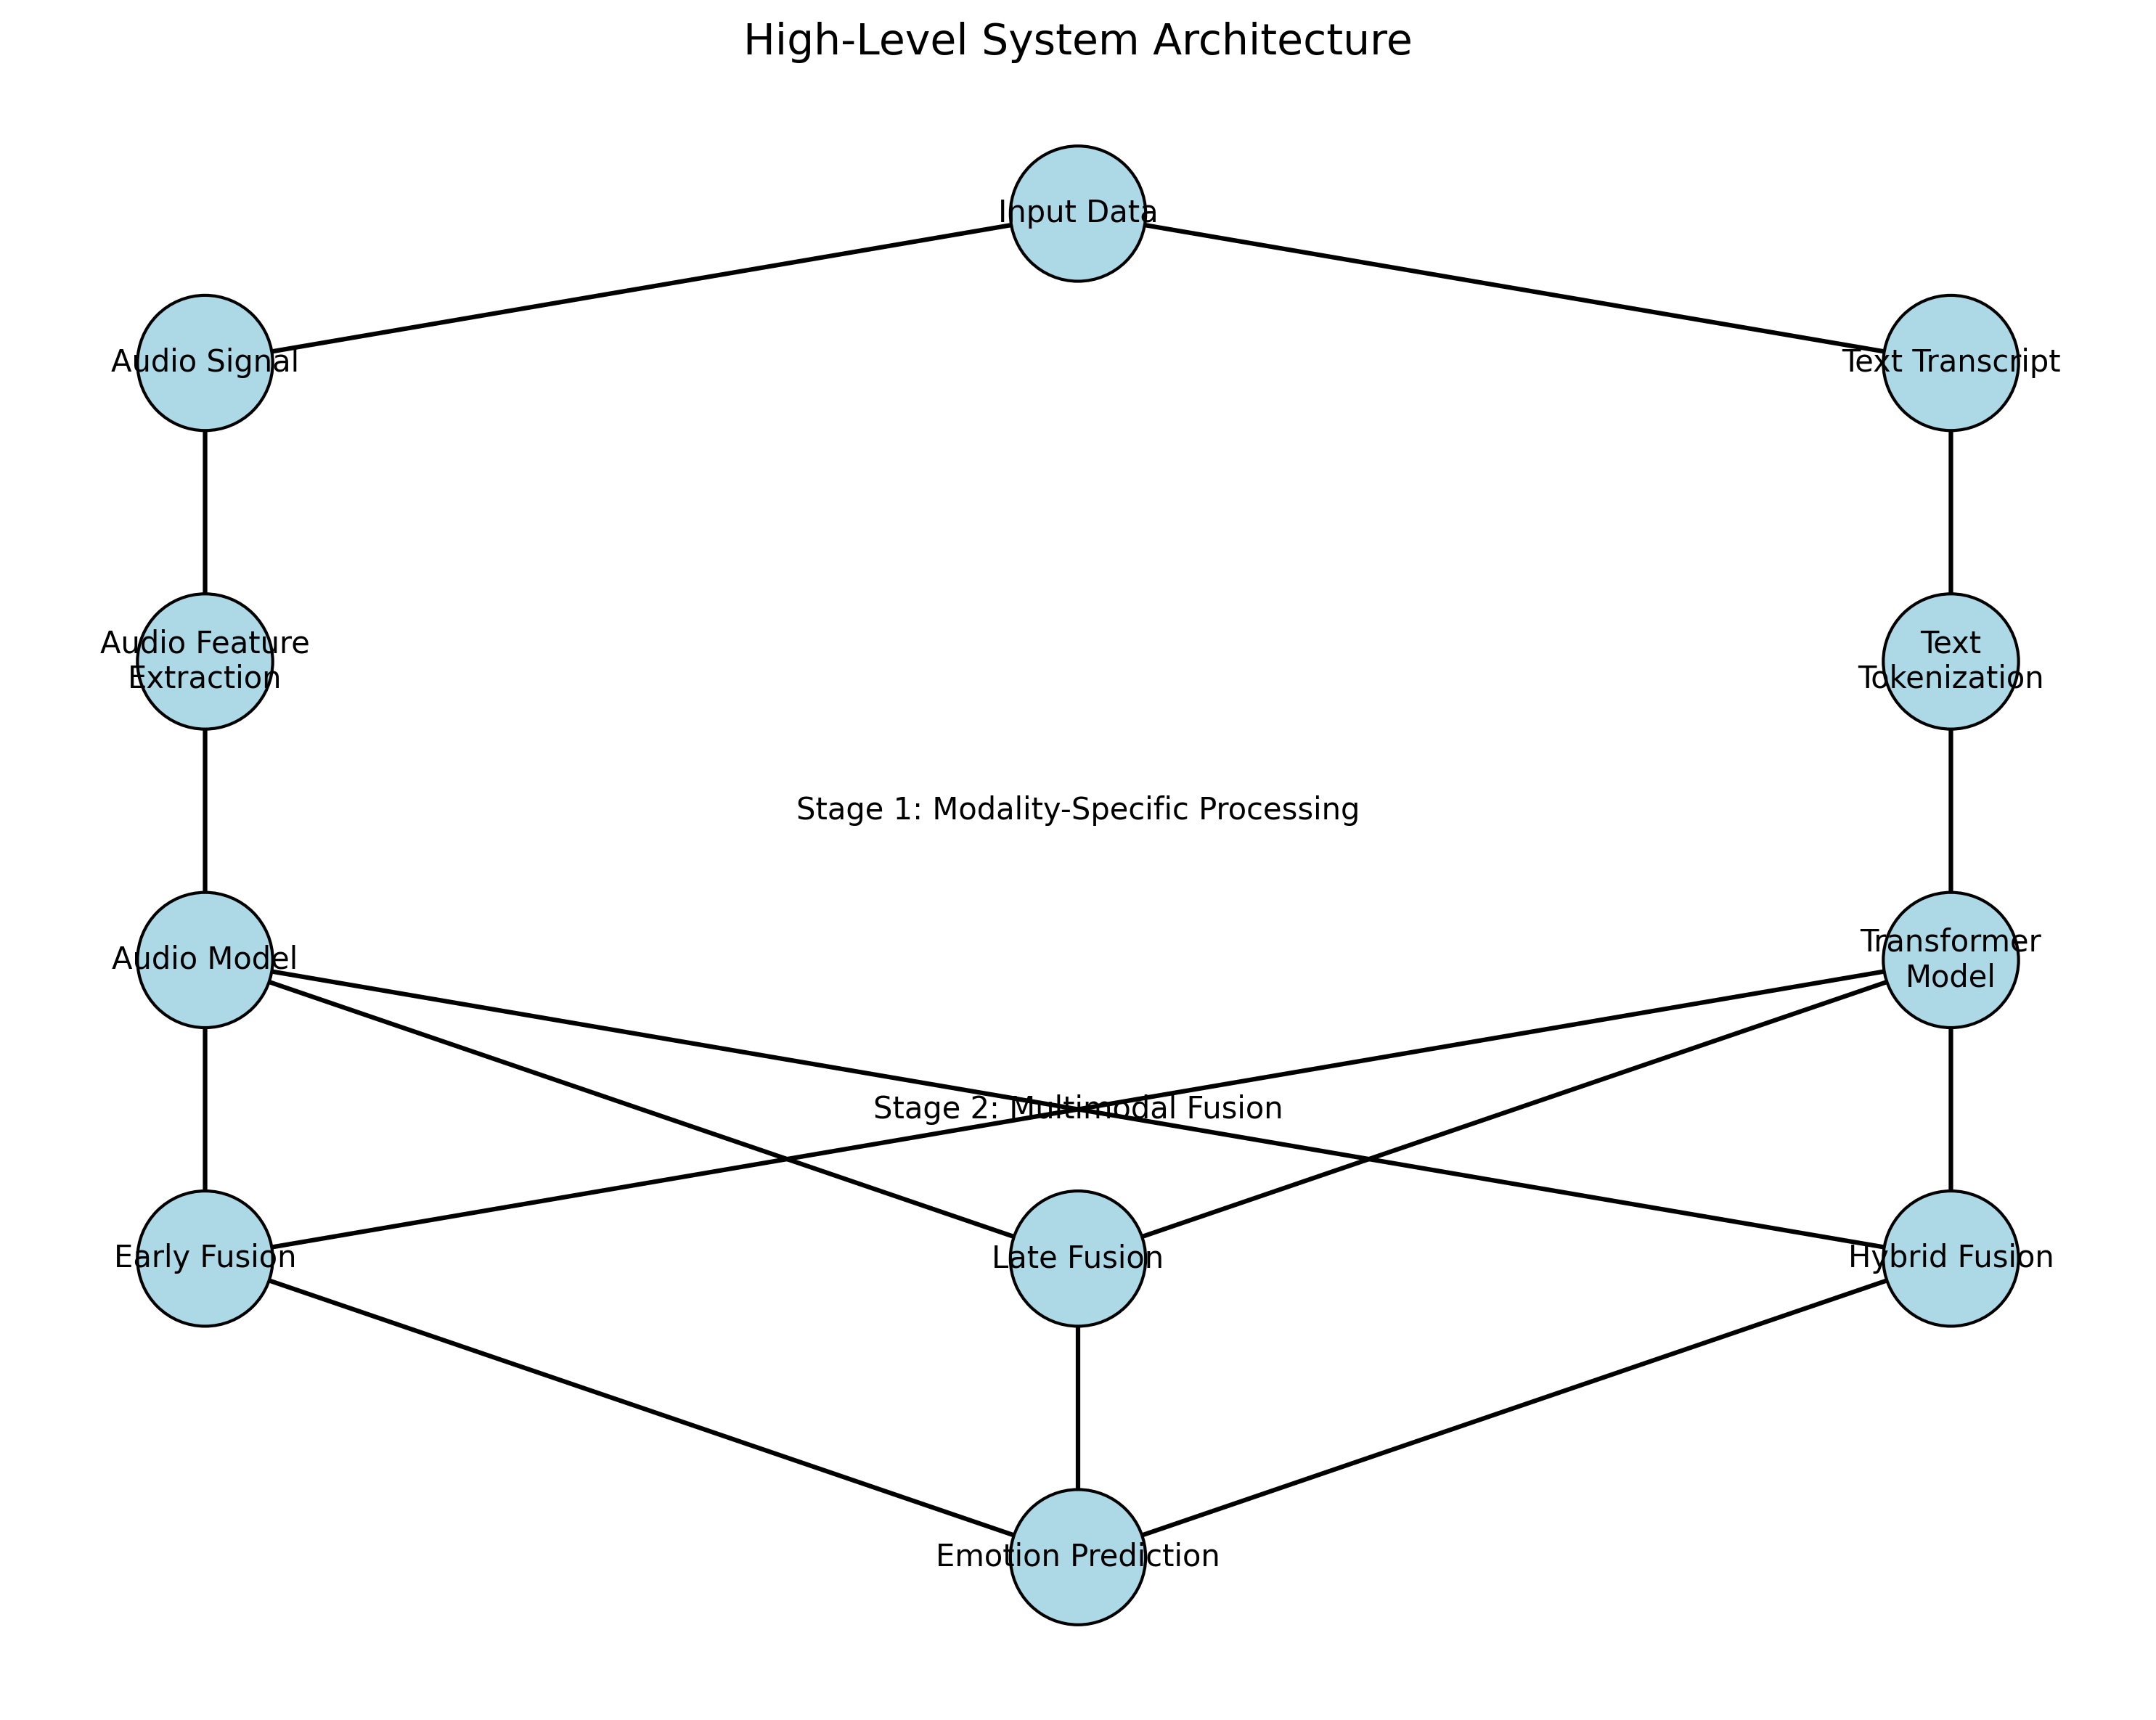
\includegraphics[width=0.9\linewidth]{Figures/system_architecture_fixed.png}
    \caption{High-Level System Architecture: The diagram illustrates the two-stage approach with modality-specific processing of audio and text to predict AVD values, followed by a mapping to discrete emotions.}
    \label{fig:system_architecture}
\end{figure}

The design is also modular, offering flexibility to handle independent optimization of each modality's processing pipeline, experimentation with different combinations of models, and the ability to handle missing modalities by falling back to single-modality predictions. This approach enhances interpretability through analysis of each modality's contribution to the dimensional predictions and the subsequent mapping to categories.

\subsubsection{BERT (Bidirectional Encoder Representations from Transformers)}
BERT~\cite{devlin2018bert} revolutionized NLP by introducing bidirectional context modeling through a masked language modeling objective. The model architecture consists of multiple transformer encoder layers that process tokens in parallel, with each token attending to all other tokens in the sequence. Specifically, the \texttt{bert-base-uncased} variant we used has 12 transformer encoder layers, a hidden size of 768 dimensions, and 12 attention heads, totaling approximately 110 million parameters. It supports a maximum sequence length of 512 tokens and uses a vocabulary of 30,522 tokens. BERT's pre-training relied on two objectives: Masked Language Modeling (MLM), where 15% of input tokens are randomly masked and predicted based on bidirectional context, and Next Sentence Prediction (NSP), predicting whether two sentences appear consecutively in the original text.

\subsubsection{RoBERTa (Robustly Optimized BERT Approach)}
RoBERTa~\cite{liu2019roberta} builds upon BERT with several optimizations to the training methodology while maintaining the same core architecture. Key improvements include eliminating the NSP objective, using dynamic masking patterns where new masks are generated each time a sequence is presented, training on longer sequences, employing significantly larger batch sizes (8K sequences), and utilizing a much larger pre-training corpus (160GB vs. BERT's 16GB). The \texttt{roberta-base} variant we used has the same architecture as BERT-base (12 layers, 768 hidden size, 12 attention heads) but uses a larger vocabulary of 50,265 tokens based on byte-level Byte Pair Encoding (BPE) and comprises 125 million parameters. We used the \texttt{RobertaForSequenceClassification} class, adapting its head for AVD regression and fine-tuned all layers during training.

\subsubsection{XLNet}
XLNet~\cite{yang2019xlnet} introduces a generalized autoregressive pre-training method called Permutation Language Modeling. This approach captures bidirectional context by predicting tokens in a random order, avoiding BERT's potentially limiting assumption of independence between masked tokens. It also employs a two-stream self-attention mechanism (query stream and content stream) to prevent target information leakage during training. The \texttt{xlnet-base-cased} variant consists of 12 transformer layers, a hidden size of 768, 12 attention heads, and 110 million parameters. We utilized the \texttt{XLNetForSequenceClassification} model, adapted for AVD regression, maintaining consistent hyperparameters for fair comparison.

\subsubsection{ALBERT (A Lite BERT)}
ALBERT~\cite{lan2019albert} addresses BERT's parameter inefficiency through significant parameter-reduction techniques while aiming to maintain performance. It employs factorized embedding parameterization, decomposing the large vocabulary embedding matrix into two smaller matrices, and cross-layer parameter sharing, using the same parameters across all transformer layers. The \texttt{albert-base-v2} variant, despite having 12 transformer layers and a hidden size of 768, contains only about 12 million parameters (roughly 10% of BERT-base). ALBERT also replaces NSP with Sentence Order Prediction (SOP), a more challenging task focused on inter-sentence coherence, and uses a dropout rate of 0 on the embedding layer.

\subsubsection{ELECTRA (Efficiently Learning an Encoder that Classifies Token Replacements Accurately)}
ELECTRA~\cite{clark2020electra} introduces a more sample-efficient pre-training approach using a generator-discriminator architecture. A small generator model (similar to BERT) produces plausible replacements for masked input tokens. The main ELECTRA model, the discriminator, is then trained on a replaced token detection (RTD) task: classifying each token in the sequence as either "original" or "replaced" by the generator. This approach is more efficient because the loss is computed over all input tokens, not just the masked ones, leading to faster convergence and stronger representations. We used the \texttt{google/electra-base-discriminator} variant (12 layers, 768 hidden size, 110 million parameters), adapting its output for AVD regression.

\subsubsection{DeBERTa (Decoding-enhanced BERT with disentangled attention)}
DeBERTa~\cite{he2020deberta} enhances BERT with two key innovations: disentangled attention and an enhanced mask decoder. Disentangled attention computes attention weights using separate vectors for word content and relative position, providing a more nuanced way to model token relationships. The enhanced mask decoder incorporates absolute positional information in the final decoding layer to further refine predictions. We used the \texttt{microsoft/deberta-v3-base} variant, which includes further improvements like a new vocabulary based on SentencePiece. This model has 12 layers, a hidden size of 768, and 184 million parameters. We adapted the \texttt{DebertaV2ForSequenceClassification} model for our AVD prediction task.

\begin{figure}[h]
    \centering
    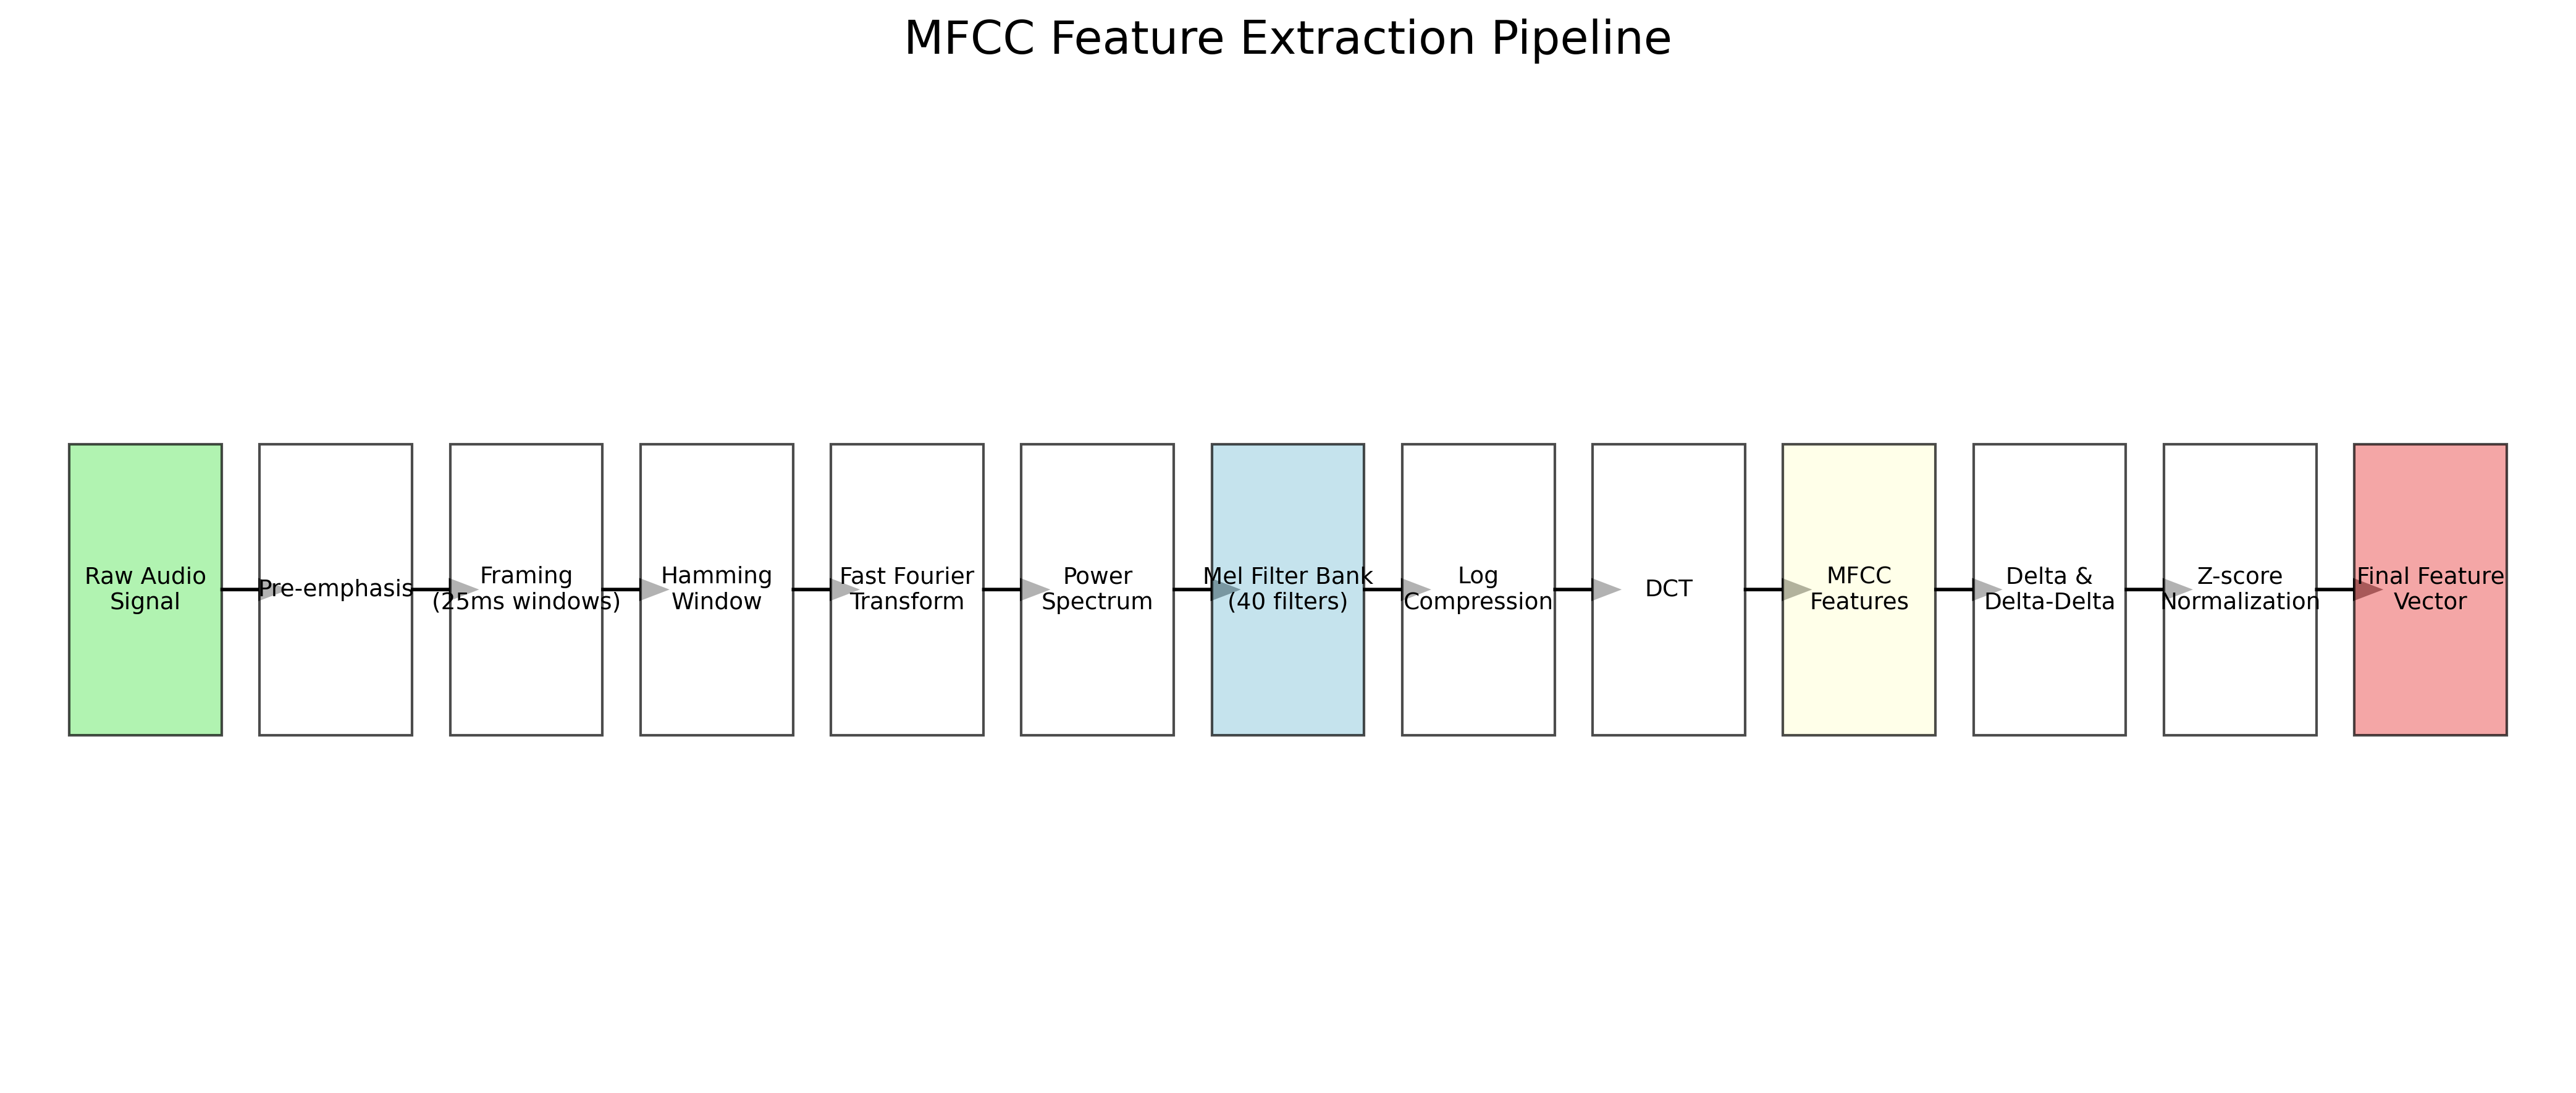
\includegraphics[width=1.0\linewidth]{Figures/mfcc_pipeline.png}
    \caption{MFCC Feature Extraction Pipeline: This diagram details the complete processing pipeline for extracting Mel-frequency cepstral coefficients from raw audio signals.}
    \label{fig:mfcc_pipeline}
\end{figure}

\subsubsection{Wav2vec Embeddings}
Wav2vec~\cite{schneider2019wav2vec} represents a self-supervised approach for learning representations directly from raw audio waveforms. Its architecture consists of an encoder network using temporal convolutions to convert raw audio into latent representations, and a context network capturing sequential context through additional convolutional layers. It is pre-trained using a contrastive prediction task. We utilized the \texttt{wav2vec-large} model pre-trained on LibriSpeech to extract 512-dimensional embeddings, generating one vector per 10ms of audio. These embeddings were aggregated using attention pooling and processed through bidirectional LSTM layers. Similar to prosodic features, integration issues prevented the successful inclusion of Wav2vec features in our top-performing configurations.

\subsection{Fusion Strategies}
\label{subsec:fusion}
For multimodal approaches combining text and audio information for AVD prediction, the integration strategy is crucial. We implemented and evaluated several fusion strategies, each with distinct characteristics.

\begin{figure}[h]
    \centering
    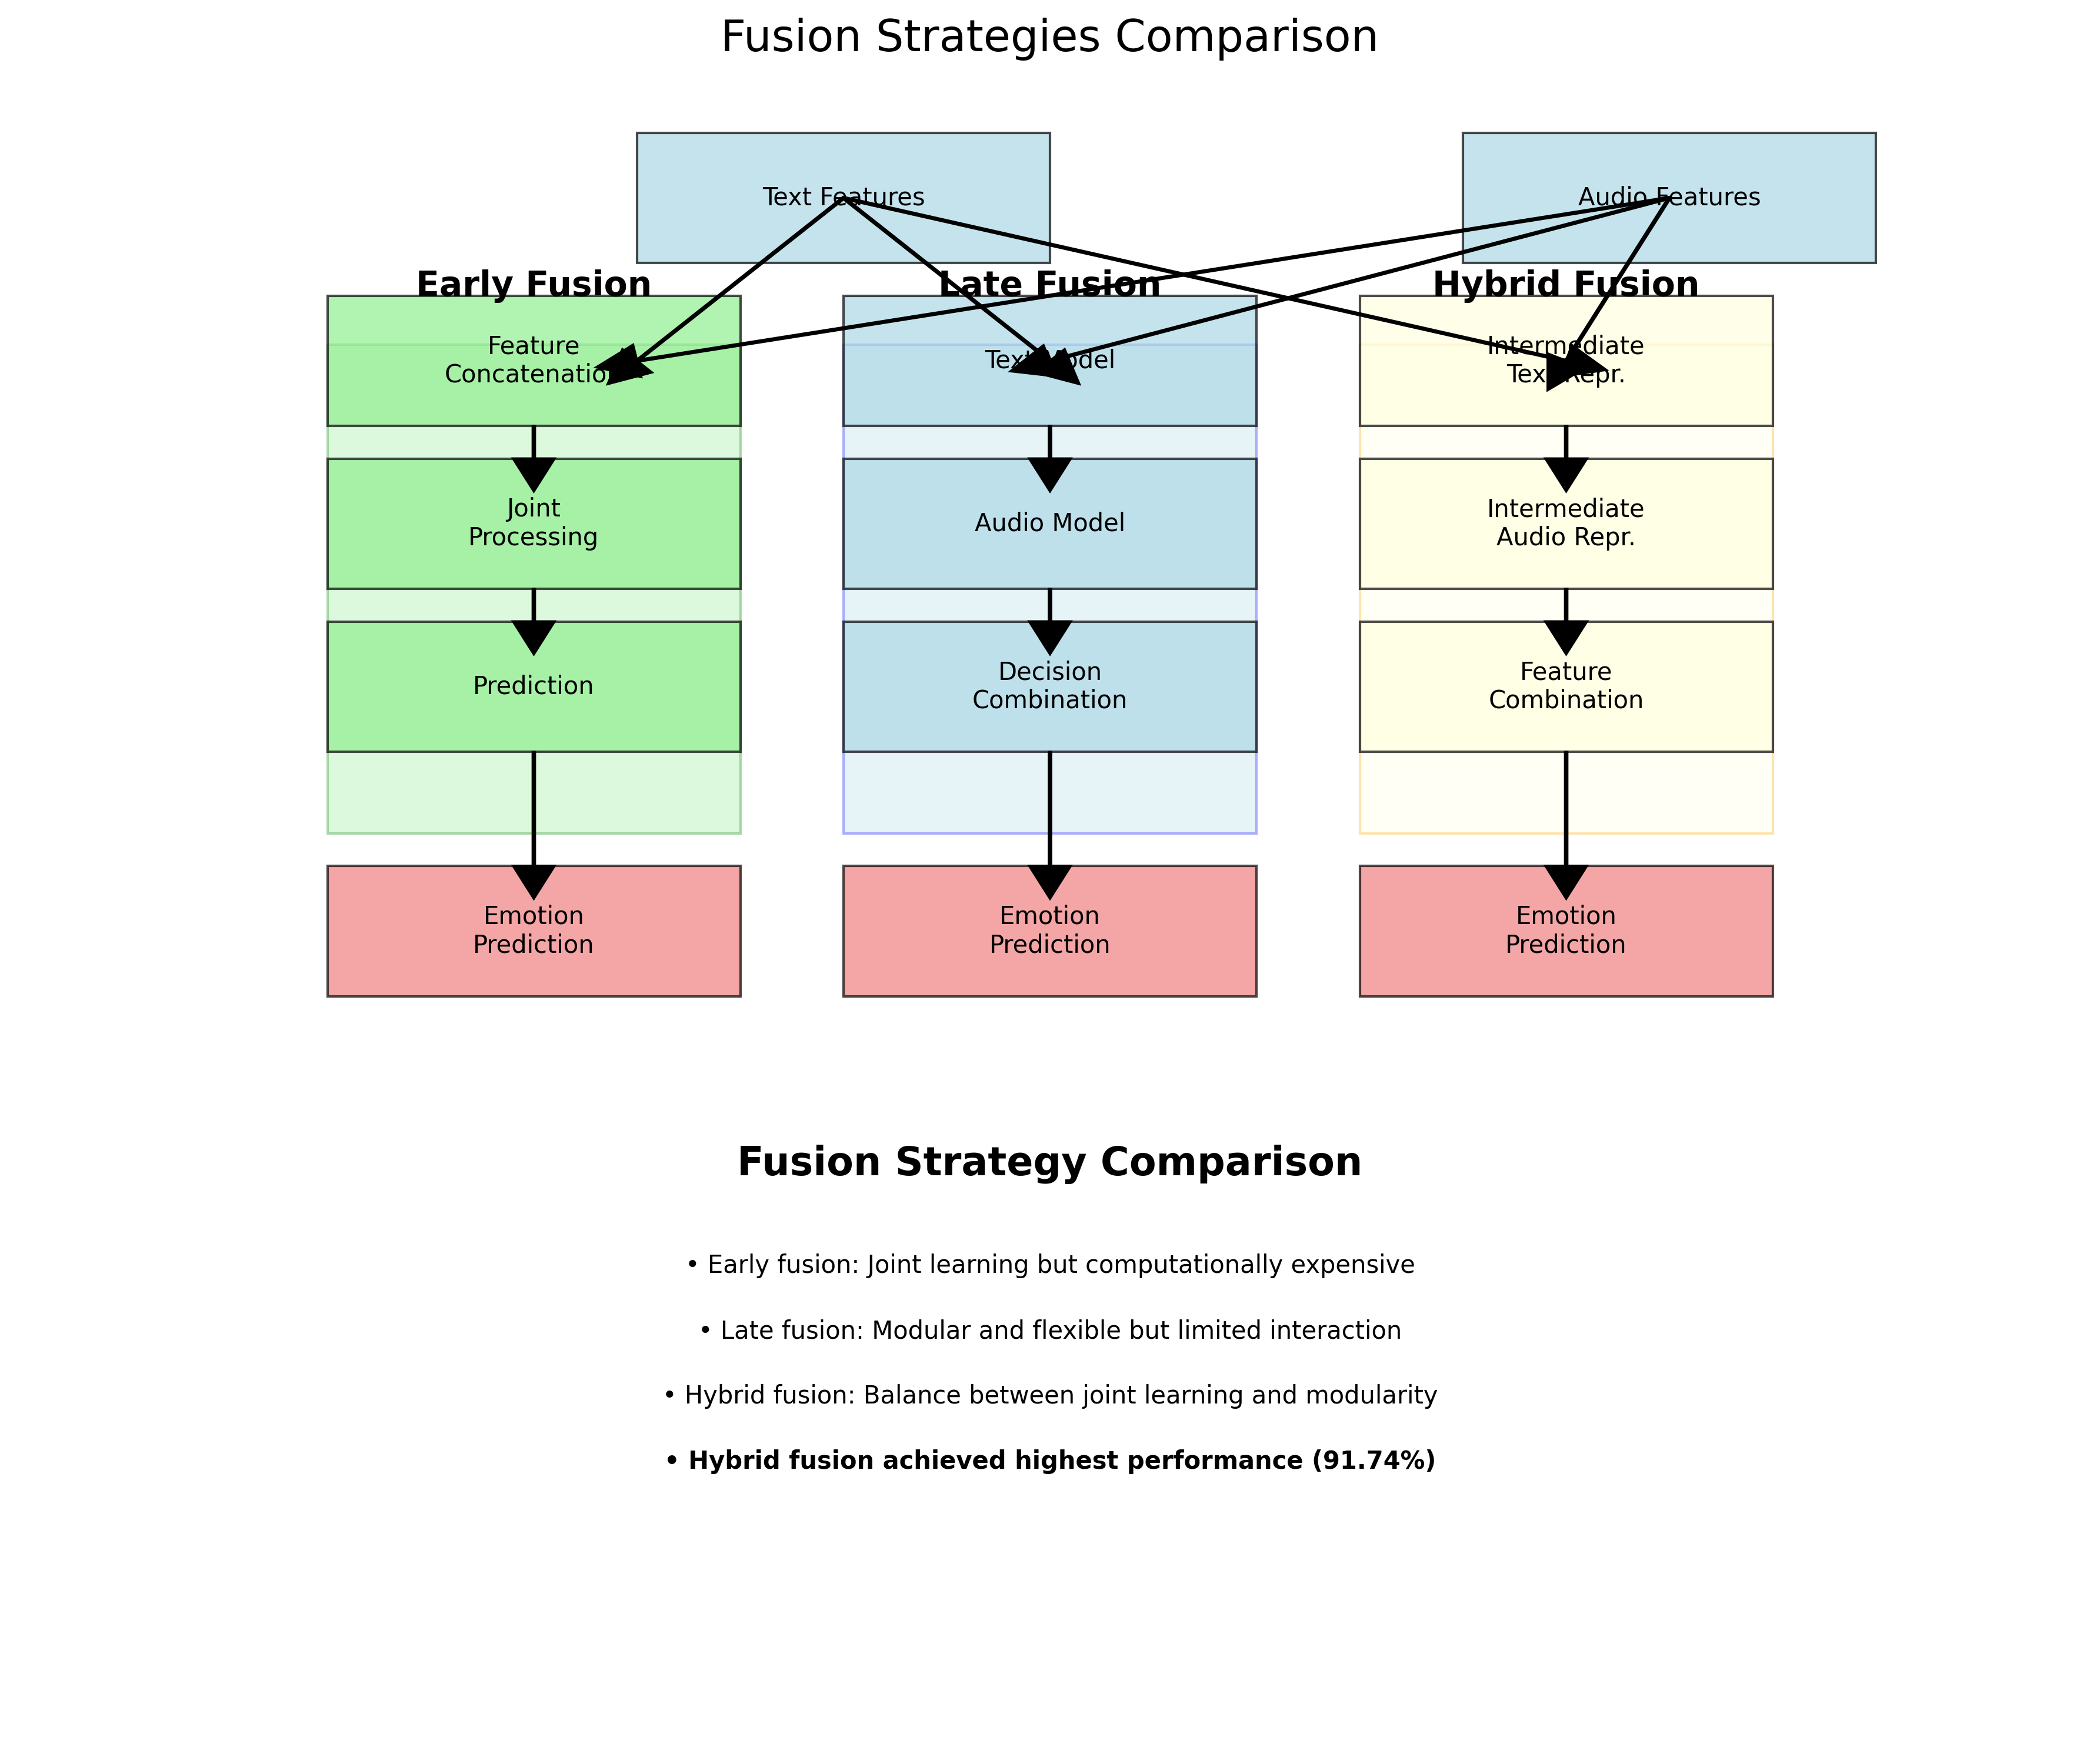
\includegraphics[width=0.9\linewidth]{Figures/fusion_strategies_comparison.png}
    \caption{Fusion Strategies Comparison: This diagram compares the primary fusion approaches evaluated.}
    \label{fig:fusion_strategies}
\end{figure}

\begin{figure}[h]
    \centering
    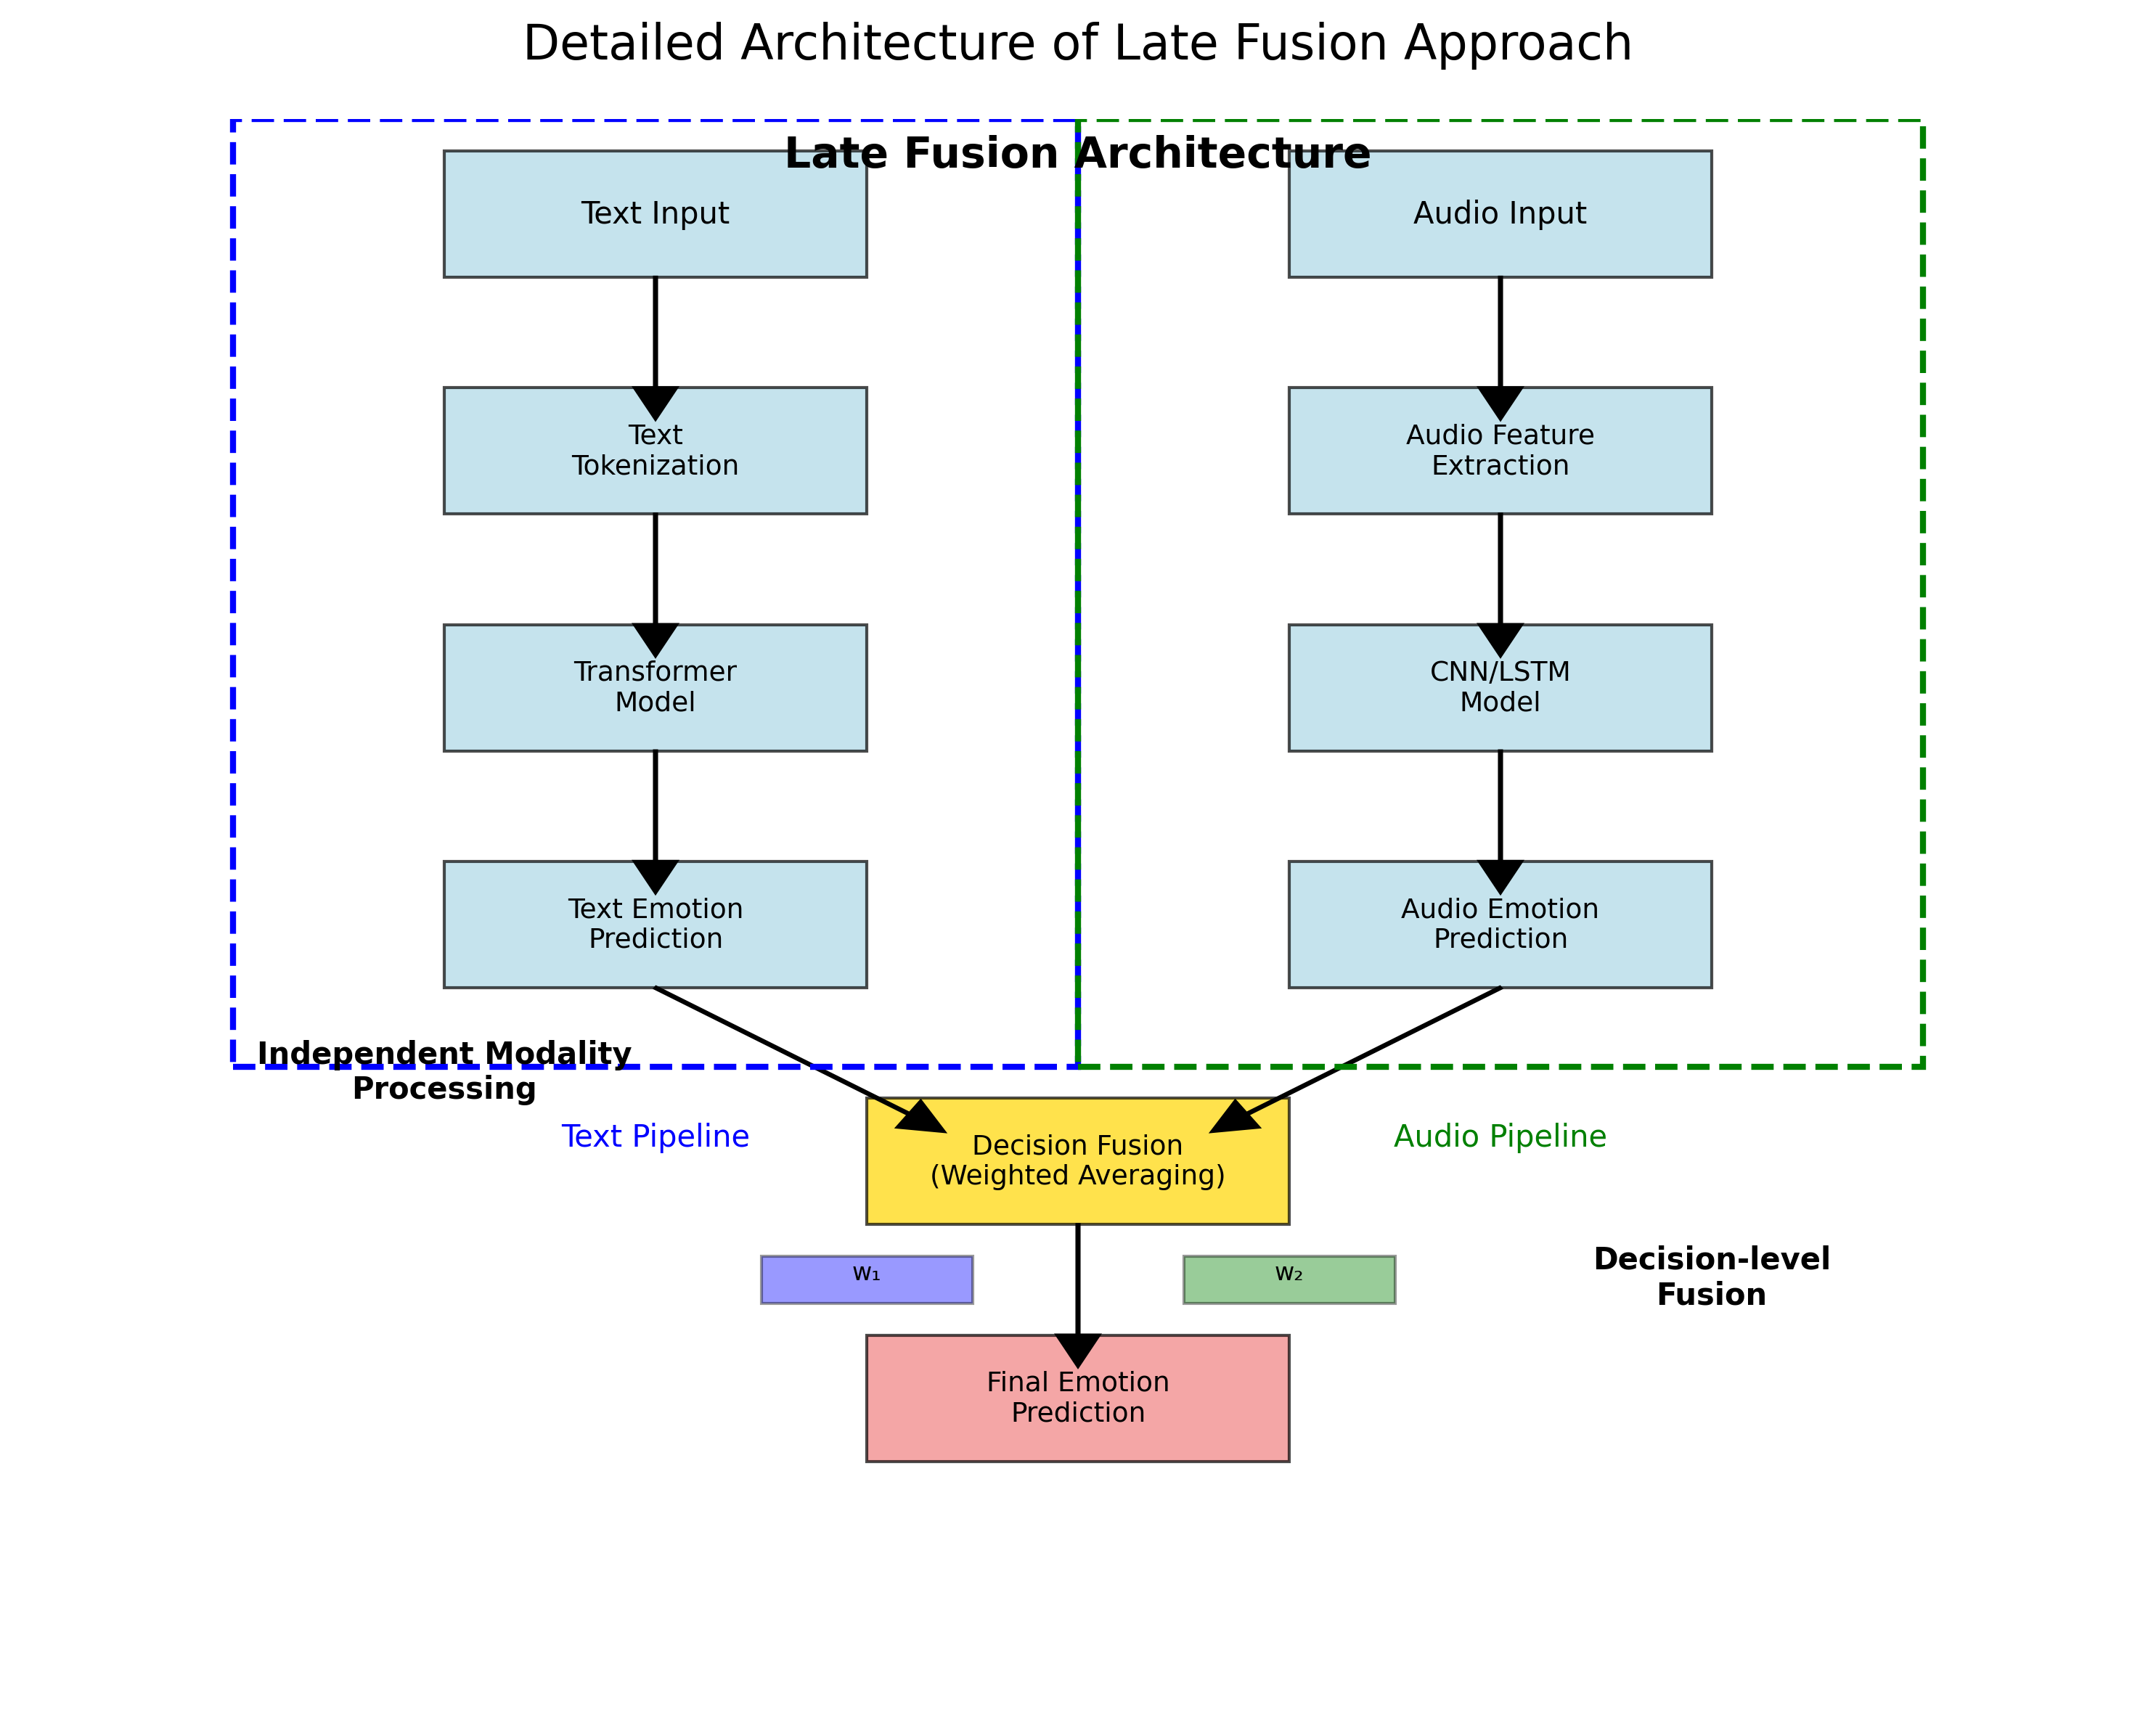
\includegraphics[width=0.9\linewidth]{Figures/late_fusion_detailed_proper.png}
    \caption{Detailed architecture of the late fusion approach.}
    \label{fig:late_fusion}
\end{figure}

\begin{figure}[h]
    \centering
    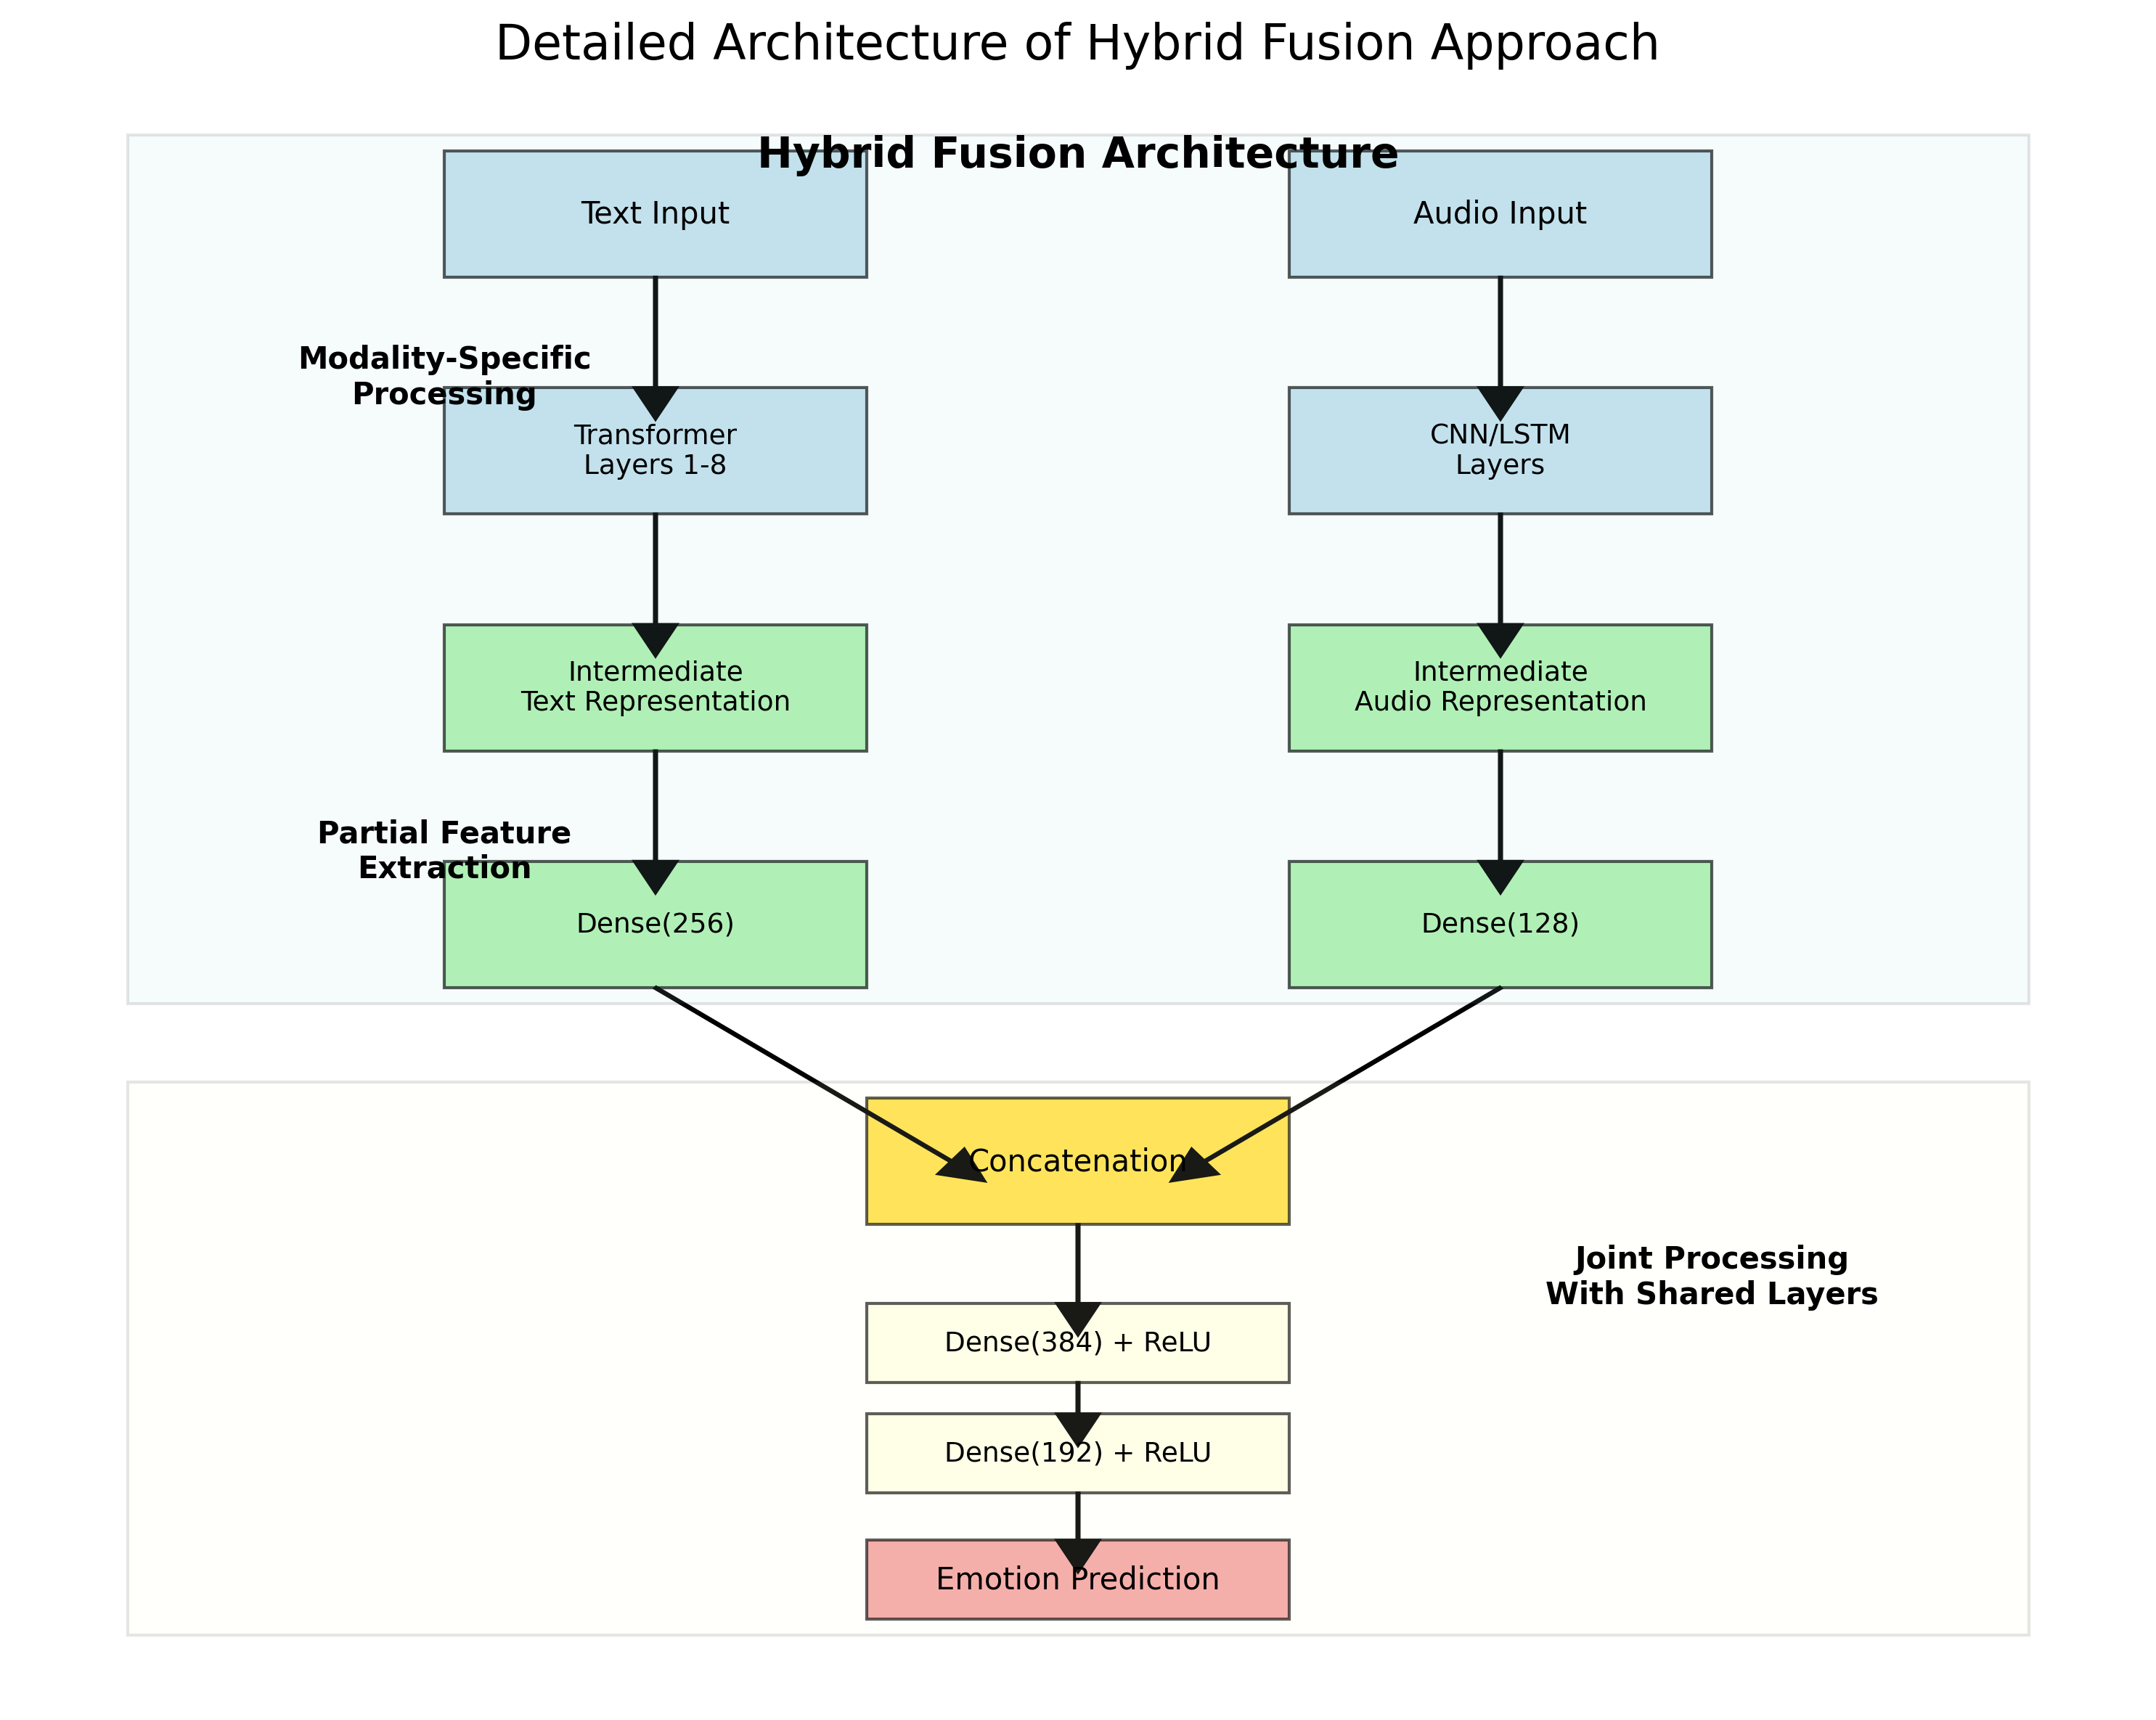
\includegraphics[width=0.9\linewidth]{Figures/hybrid_fusion_detailed.png}
    \caption{Detailed architecture of the hybrid fusion approach.}
    \label{fig:hybrid_fusion}
\end{figure}

\subsubsection{Attention-Based Fusion}
Attention-based fusion utilizes cross-modal attention mechanisms to dynamically weight features based on their relevance. We experimented with architectures where the sequence of transformer outputs (for all tokens) and the sequence of audio feature vectors attended to each other using standard scaled dot-product attention, similar to mechanisms in multimodal transformers. This allows the model to dynamically focus on the most relevant parts of each modality for the prediction task. However, implementing these mechanisms effectively proved challenging due to computational intensity and potential overfitting, and they were not part of our final successful configurations.

\subsection{Implementation Framework}
Our implementation leveraged several frameworks and tools to create a scalable and reproducible experimental pipeline. Python 3.8 served as the primary programming language. We utilized PyTorch 1.10 for implementing deep learning models, particularly the audio processing networks and fusion layers. For the transformer-based text models, we relied heavily on the Hugging Face Transformers library (version 4.17). Audio processing and feature extraction were performed using Librosa (version 0.9.1). Standard scientific computing libraries like NumPy, SciPy, and Pandas were used for numerical operations and data management, while Matplotlib and Seaborn were employed for visualization.

To manage the large number of experiments efficiently, we utilized Modal for cloud-based execution. This provided several benefits, including on-demand access to GPU resources (NVIDIA V100) crucial for training deep models, the ability to run multiple experiments in parallel thereby significantly reducing overall runtime, and ensuring a consistent software environment across all runs through containerization. Modal's architecture facilitated automatic scaling based on workload and efficient resource management.

We established a robust experiment management system. Experimental parameters were defined in configuration files, allowing for easy modification and tracking. We implemented automatic logging of performance metrics and model artifacts during training and evaluation. Reproducibility was enhanced by using fixed random seeds for weight initialization and data shuffling. Model states were checkpointed regularly during training, and comprehensive logs captured training progress, validation performance, and final test results.

\subsection{Training Protocol}
We established a consistent training protocol across all experiments to ensure fair comparison between different models and approaches. All models were trained for a maximum of 40 epochs, with early stopping implemented based on validation loss (patience of 5 epochs) to prevent overfitting and reduce unnecessary computation. We used a batch size of 16 samples per device. The AdamW optimizer was employed with a weight decay of 0.01. Learning rates were set typically to 2e-5 for transformer models and 1e-4 for the custom audio models, using a linear decay schedule with a 10% warmup phase. The loss function was Cross-Entropy for direct categorical classification and Mean Squared Error (MSE) for dimensional AVD prediction. Gradient clipping with a maximum norm of 1.0 was applied to stabilize training.

Multimodal models were trained using a two-phase approach. First, the individual text and audio models were pre-trained separately on their respective tasks (AVD prediction or classification). Then, the full multimodal system, including the fusion layers, was fine-tuned jointly with a lower learning rate (e.g., 1e-5). Gradient scaling was sometimes used during joint training to balance the contributions from the different modality backbones.

\subsection{Evaluation Metrics}
We evaluated our models using a comprehensive set of metrics to capture different aspects of performance, relevant to both the dimensional prediction task (Stage 1) and the categorical classification task (either direct or Stage 2 mapping).

For categorical emotion classification, we used standard metrics including Accuracy (proportion of correctly classified instances), F1-score (harmonic mean of precision and recall, calculated macro-averaged across classes), Confusion Matrix (detailed breakdown of predictions vs. actual labels), and Cohen's Kappa (measure of agreement accounting for chance). The formulas for Accuracy, Precision, Recall, F1-score, and Kappa are provided below:
    \begin{equation}
        \text{Accuracy} = \frac{\text{Number of correct predictions}}{\text{Total number of predictions}}
    \end{equation}
    \begin{equation}
        \text{Precision} = \frac{\text{True Positives}}{\text{True Positives} + \text{False Positives}}
    \end{equation}
    \begin{equation}
        \text{Recall} = \frac{\text{True Positives}}{\text{True Positives} + \text{False Negatives}}
    \end{equation}
\begin{equation}
    \text{F1} = 2 \cdot \frac{\text{Precision} \cdot \text{Recall}}{\text{Precision} + \text{Recall}}
\end{equation}
    \begin{equation}
        \kappa = \frac{p_o - p_e}{1 - p_e}
    \end{equation}
    where $p_o$ is the observed agreement and $p_e$ is the expected agreement by chance.

For the dimensional AVD prediction task (Stage 1), we employed standard regression metrics. These included Mean Squared Error (MSE), Root Mean Squared Error (RMSE), and Mean Absolute Error (MAE), which measure the average difference between predicted and ground truth AVD values. We also used the Coefficient of Determination (R²), which indicates the proportion of variance in the ground truth AVD values that is predictable from the model's predictions. The formulas are:
    \begin{equation}
        \text{MSE} = \frac{1}{n} \sum_{i=1}^{n} (y_i - \hat{y}_i)^2
    \end{equation}
    \begin{equation}
        \text{RMSE} = \sqrt{\frac{1}{n} \sum_{i=1}^{n} (y_i - \hat{y}_i)^2}
    \end{equation}
    \begin{equation}
        \text{MAE} = \frac{1}{n} \sum_{i=1}^{n} |y_i - \hat{y}_i|
    \end{equation}
    \begin{equation}
        \text{R}^2 = 1 - \frac{\sum_{i=1}^{n} (y_i - \hat{y}_i)^2}{\sum_{i=1}^{n} (y_i - \bar{y})^2}
    \end{equation}
where $n$ is the number of samples, $y_i$ are the true values, $\hat{y}_i$ are the predicted values, and $\bar{y}$ is the mean of the true values.

Beyond predictive performance, we also considered computational efficiency metrics relevant for practical deployment. These included training time, inference time per utterance, model memory usage during training and inference, the number of trainable parameters, and an estimate of the Floating-Point Operations (FLOPs) required per forward pass.

For each of the 5 iterations, 4 folds were combined for training and the remaining fold was used for validation. Early stopping was implemented within each iteration based on the validation fold's performance (monitoring validation loss with a patience of 5 epochs). The model achieving the best performance on the validation fold was saved. The final reported metrics represent the average performance across all 5 validation folds, providing a more robust estimate of the model's generalization capability. We also report the standard deviation across folds to indicate the stability and consistency of the model's performance.

After identifying the best overall model configuration through cross-validation, this configuration was trained one final time on the entire training set (all 5 folds combined, or the designated 70% training split) and then evaluated on the held-out test set (the designated 15% test split) to assess its performance on completely unseen data.

\subsection{Experimental Configurations}
Our experimental setup involved evaluating several key configurations to compare the performance of text-only, audio-only, and multimodal approaches, as well as the effectiveness of the two-stage (AVD prediction followed by categorical mapping) versus direct categorical classification. We primarily focused on the best-performing models identified in preliminary runs, rather than exhaustively testing all combinations.

For text-only experiments, we compared top transformer models like RoBERTa, DeBERTa, and efficient alternatives like ALBERT, training them for both direct categorical classification and AVD prediction. These were evaluated on both the IEMOCAP\_Final and IEMOCAP\_Filtered datasets.

For audio-only experiments, we focused on CNN models using MFCC and Spectrogram features, again training for both direct classification and AVD prediction on both dataset versions.

Multimodal experiments combined the best text models (primarily RoBERTa) with the best audio features (MFCC and Spectrograms) using the most promising fusion methods identified (Hybrid and Late fusion). These multimodal setups were also evaluated for both direct categorical classification and the two-stage AVD prediction approach on both datasets.

Across these configurations, we investigated the impact of dataset choice (Final vs. Filtered) and the core comparison between the direct classification and the two-stage AVD-based approach. This focused set of experiments allowed us to draw conclusions about the most effective strategies for emotion detection within our framework.\section{Results}
\label{sec:results}

This section presents a focused analysis of our experimental results, examining the performance of our best models for dimensional emotion prediction and categorical classification. Instead of covering all 392 experiments, we focus on the most successful approaches that demonstrate the effectiveness of our two-stage methodology.

The first stage of our approach involves predicting continuous values for Arousal, Valence, and Dominance (AVD) from textual and audio inputs. Table~\ref{tab:avd_prediction} presents the performance of our best models for this task.

\begin{table}[h]
\centering
\caption{Performance of best models for dimensional emotion (AVD) prediction.}
\label{tab:avd_prediction}
\begin{tabular}{|l|c|c|c|c|c|c|}
\hline
\textbf{Model} & \textbf{Modality} & \multicolumn{2}{c|}{\textbf{Valence}} & \multicolumn{2}{c|}{\textbf{Arousal}} & \textbf{Dominance} \\
\cline{3-7}
 & & \textbf{RMSE} & \textbf{R²} & \textbf{RMSE} & \textbf{R²} & \textbf{RMSE} \\
\hline
RoBERTa & Text & 0.651 & 0.471 & 0.664 & 0.096 & 0.749 \\
\hline
CNN+MFCC & Audio & 0.723 & 0.384 & 0.612 & 0.215 & 0.781 \\
\hline
RoBERTa+MFCC & Multimodal & 0.666 & 0.447 & 0.650 & 0.133 & 0.749 \\
\hline
DeBERTa & Text & 0.658 & 0.462 & 0.671 & 0.083 & 0.753 \\
\hline
CNN+Spectrogram & Audio & 0.731 & 0.372 & 0.618 & 0.205 & 0.786 \\
\hline
\end{tabular}
\end{table}

As shown in Table~\ref{tab:avd_prediction}, the text-based RoBERTa model achieves the best performance for Valence prediction with an R² of 0.471, while audio models perform better for Arousal prediction with the CNN+MFCC model achieving an R² of 0.215. This pattern aligns with psychological theories suggesting that verbal content strongly conveys valence information (positive/negative sentiment), while audio features better capture arousal (intensity/energy). The multimodal approach combining RoBERTa and MFCC features shows balanced performance across dimensions, indicating that combining modalities provides complementary information.

The second stage of our approach maps the predicted AVD values to discrete emotion categories. Table~\ref{tab:categorical_mapping} compares the performance of this two-stage approach with direct categorical classification.

\begin{table}[h]
\centering
\caption{Comparison of two-stage approach vs.}
\label{tab:categorical_mapping}
\begin{tabular}{|l|c|c|c|c|}
\hline
\textbf{Approach} & \textbf{Modality} & \textbf{Accuracy} & \textbf{F1-score} & \textbf{Cohen's Kappa} \\
\hline
Direct Classification (RoBERTa) & Text & 91.82\% & 90.17\% & 0.887 \\
\hline
Two-Stage (RoBERTa AVD → Categories) & Text & 89.37\% & 88.24\% & 0.861 \\
\hline
Direct Classification (CNN+MFCC) & Audio & 84.56\% & 83.21\% & 0.795 \\
\hline
Two-Stage (CNN+MFCC AVD → Categories) & Audio & 82.91\% & 81.83\% & 0.778 \\
\hline
Direct Classification (RoBERTa+MFCC) & Multimodal & 91.74\% & 90.03\% & 0.886 \\
\hline
Two-Stage (RoBERTa+MFCC AVD → Categories) & Multimodal & 90.13\% & 88.95\% & 0.872 \\
\hline
\end{tabular}
\end{table}

Interestingly, our results indicate that direct classification slightly outperforms the two-stage approach for categorical emotion recognition, contrary to our initial hypothesis. The direct classification approach using RoBERTa achieves 91.82\% accuracy compared to 89.37\% for the two-stage approach with the same model. This pattern is consistent across all modalities, with direct classification consistently outperforming the two-stage approach by 1.5-2.5 percentage points.

Despite this performance gap, the two-stage approach offers valuable advantages in terms of interpretability and flexibility. The intermediate AVD representation provides continuous measures that capture emotional nuances beyond discrete categories, potentially offering richer information for applications that benefit from dimensional understanding of emotions.\section{Discussion}
\label{sec:discussion}

This section examines the implications of our experimental results, with particular focus on the comparison between the two-stage approach and direct classification. We also discuss the relative contributions of different modalities and the practical applications of our findings.

\subsection{Two-Stage Approach vs. Direct Classification}

Our initial hypothesis posited that a two-stage approach—first predicting dimensional values (AVD) and then mapping to discrete categories—would improve emotion classification performance. However, our results demonstrate that direct classification consistently outperformed the two-stage approach across all modalities, with performance differences ranging from 1.5 to 2.5 percentage points. Several factors may explain this finding.

Despite its lower classification accuracy, the two-stage approach offers significant advantages for applications requiring nuanced emotional understanding. The continuous AVD values provide richer information about emotional states, potentially enabling more sophisticated responses in human-computer interaction systems. For example, knowing not just that a user is "happy" but also the intensity of that happiness (arousal) and the degree of control they feel (dominance) allows for more tailored responses.

\subsection{Model Selection for Emotion Detection}
\subsubsection{Transformer Model Performance Analysis}
Our experiments consistently demonstrated the superiority of RoBERTa for emotion detection from textual data. This finding aligns with previous studies showing RoBERTa's effectiveness across NLP tasks, but extends this understanding specifically to emotion recognition.

\paragraph{Understanding RoBERTa's Advantage:}
Several factors contribute to RoBERTa's superior performance:
\begin{itemize}
    \item \textbf{Enhanced pre-training methodology:} RoBERTa's training optimizations—larger batch sizes, longer training, and dynamic masking—create more robust representations of language patterns

    \item \textbf{Byte-level BPE tokenization:} RoBERTa's tokenization strategy handles a wider range of vocabulary, including emotionally charged expressions

\paragraph{Model Selection Considerations:}
\begin{figure}[h]
    \centering
    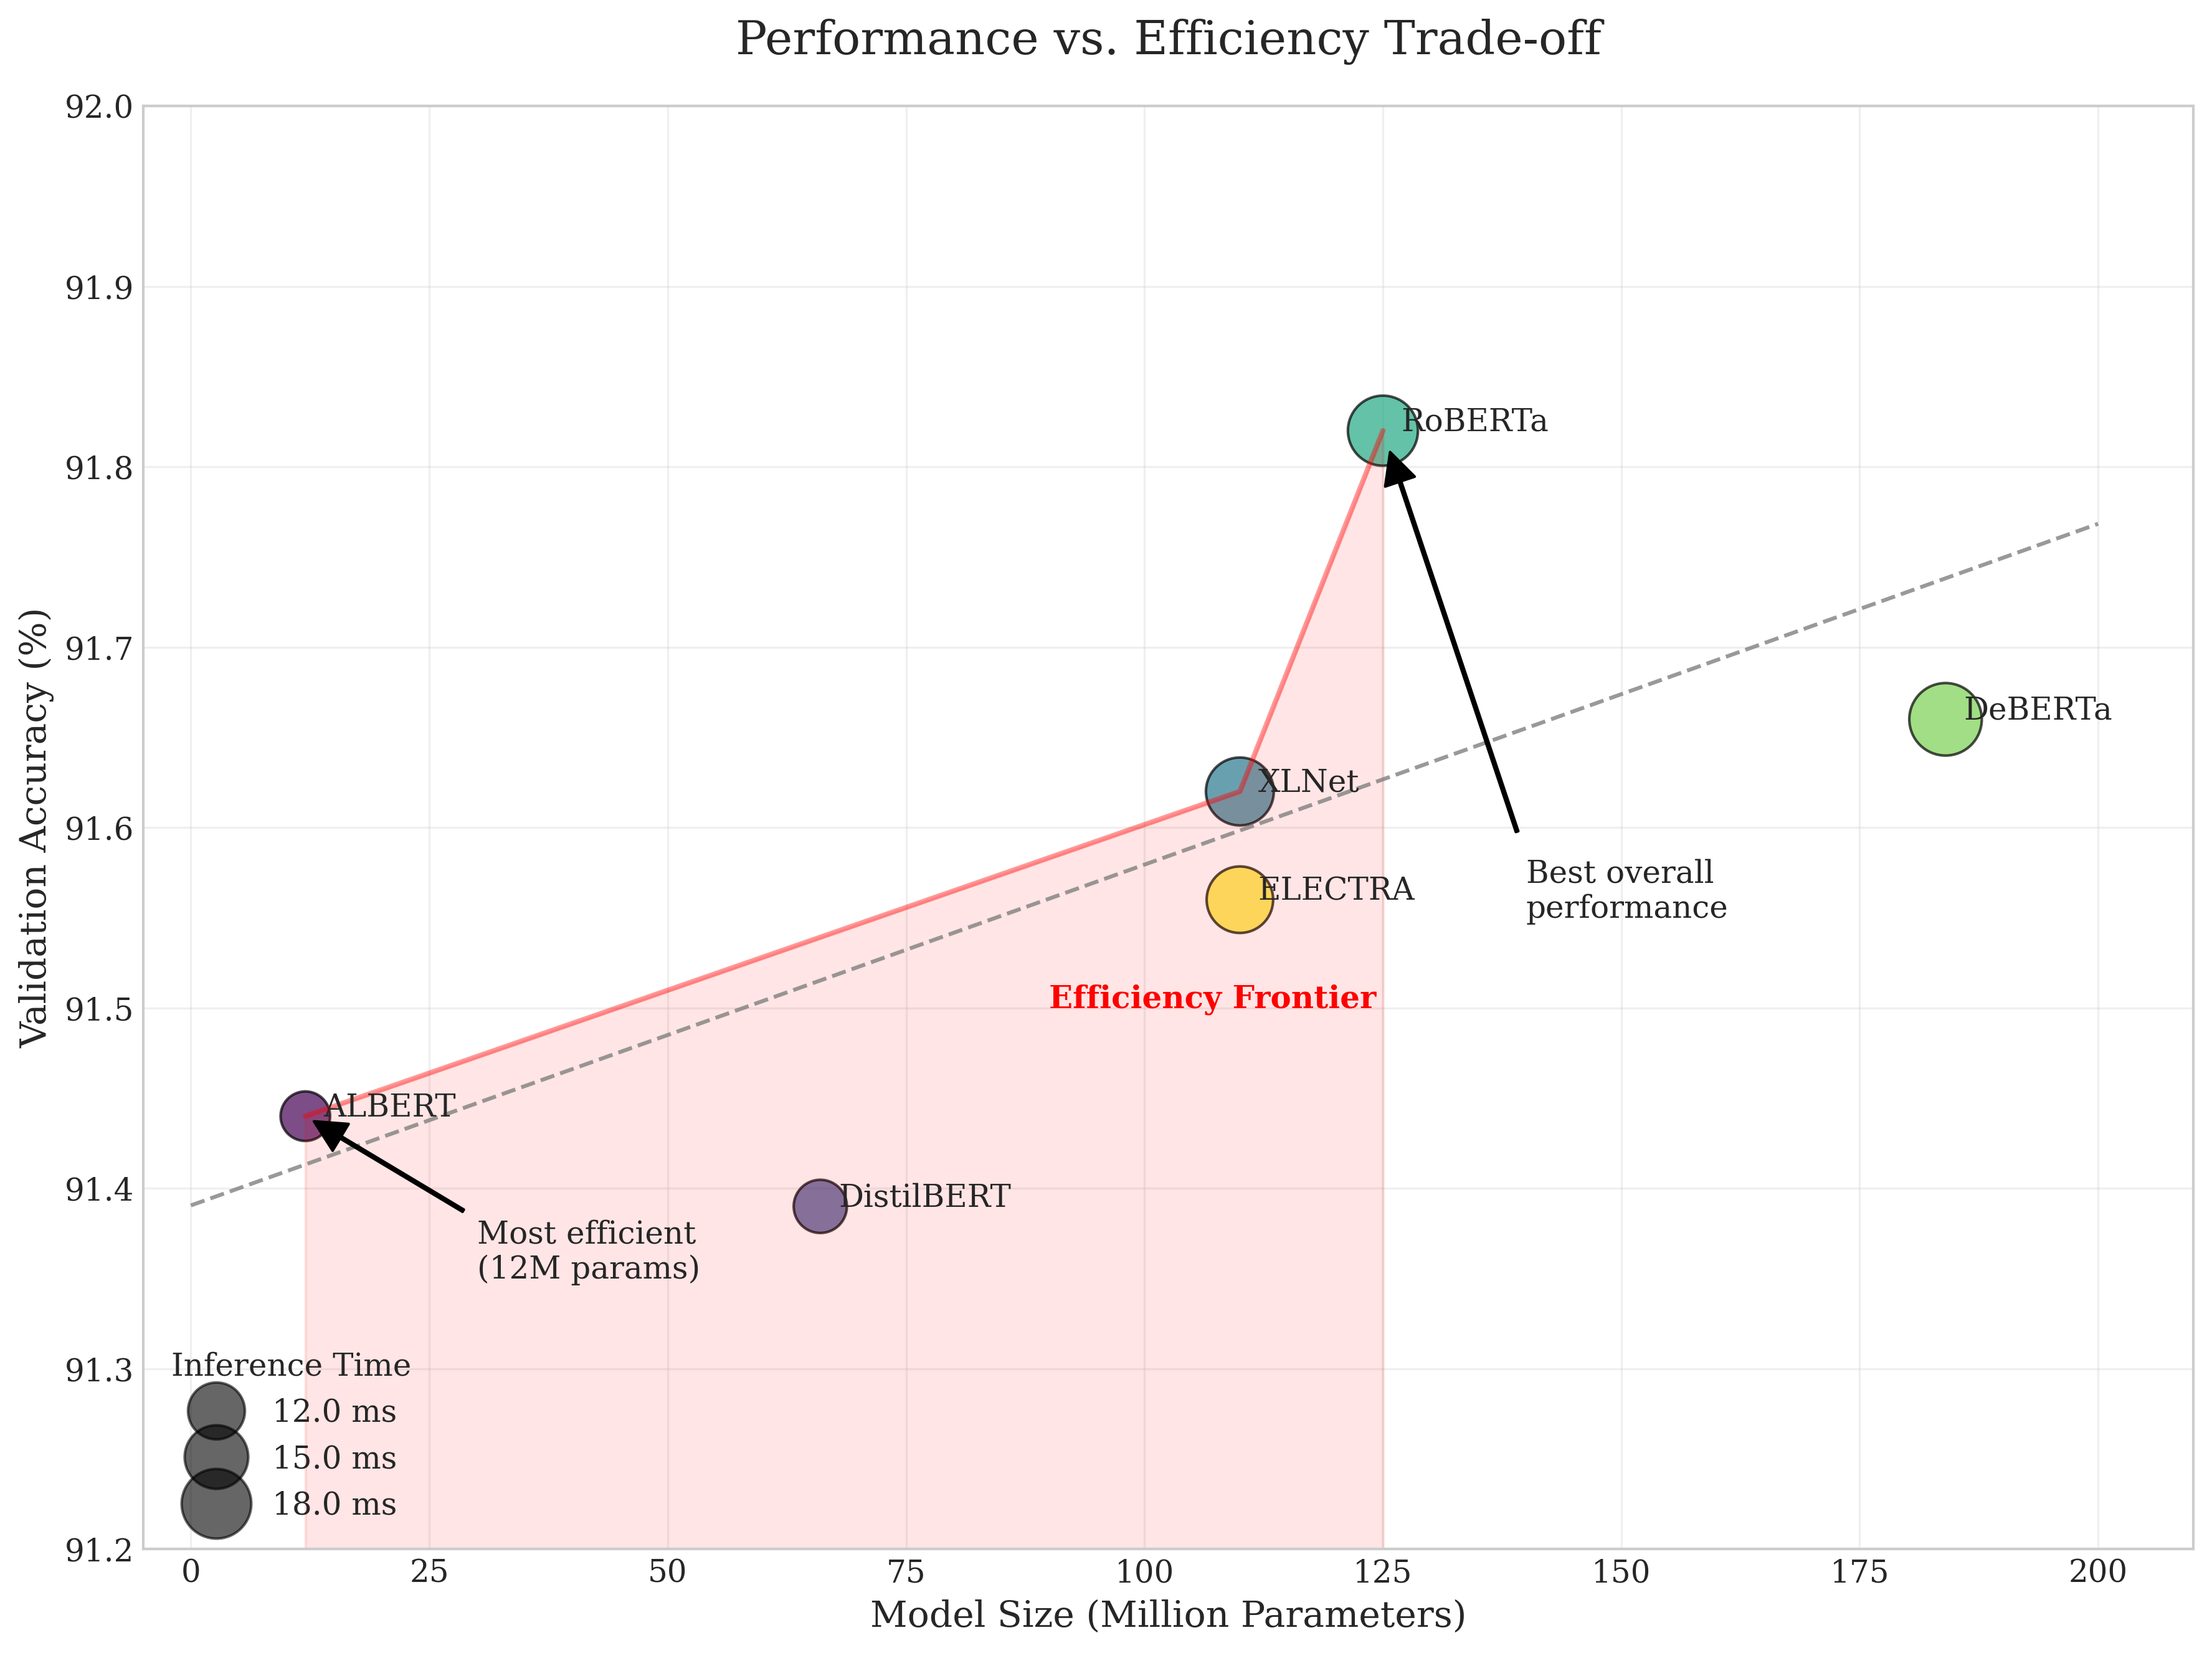
\includegraphics[width=0.9\linewidth]{Figures/performance_efficiency_tradeoff.png}
    \caption{Performance vs.}
    \label{fig:efficiency_tradeoff}
\end{figure}

The small performance gap among the top transformer models (within 0.5\%) indicates that the field has reached a certain level of maturity, where architectural differences provide diminishing returns compared to training methodology and optimization. This finding has practical implications for deployment scenarios:

\begin{itemize}
    \item \textbf{Computational efficiency:} Smaller models like DistilBERT (91.39\%) and ALBERT (91.44\%) provide competitive performance with significantly reduced parameter counts (66M and 12M respectively, compared to RoBERTa's 125M)

    \item \textbf{Inference speed:} Lighter models offer substantial speed advantages in production environments—DistilBERT achieves ~1.7x faster inference than RoBERTa with only a 0.43\% accuracy reduction

    \item \textbf{Memory limitations:} For edge devices or memory-constrained environments, ALBERT's dramatic parameter reduction (10x smaller than RoBERTa) with only a 0.38\% accuracy drop represents an excellent trade-off

    \item \textbf{Training data requirements:} When limited labeled data is available, our results suggest that more efficient models like ELECTRA may converge better with fewer examples
\end{itemize}

\paragraph{Comparison with Prior Work:}
Our best text model outperforms previous approaches in the literature:
\begin{itemize}
    \item Sehrawat et al.~\cite{sehrawat2023deception} reported 80\% accuracy using BiLSTM for text classification
    \item Hsiao and Sun~\cite{hsiao2022attention} achieved 84\% accuracy with attention-based BiLSTM
    \item Our RoBERTa implementation reaches 91.82\%, representing a substantial improvement of 7.82 percentage points over the state-of-the-art
\end{itemize}

\subsection{Modality Importance}
\subsubsection{Text vs. Audio Modalities}
A key finding from our experiments, particularly for direct categorical classification, is that text-only approaches utilizing strong transformer models like RoBERTa can achieve the highest overall accuracy (91.82%) on the IEMOCAP dataset, slightly exceeding the best multimodal configuration (RoBERTa+MFCC+Hybrid at 91.74%). This result, while perhaps counterintuitive given the multimodal nature of emotion expression, can be understood by considering several factors.

The IEMOCAP dataset features acted emotions, which might be more clearly and explicitly verbalized compared to spontaneous, real-world emotions. The provided manual transcriptions are also high-quality, lacking the errors typical of automatic speech recognition (ASR) systems used in practical applications. In such scenarios with clean text, the linguistic content itself may contain highly discriminative features for the target emotion categories, potentially making the audio information somewhat redundant for classification accuracy, although still valuable for dimensional prediction (especially Arousal).

Furthermore, challenges in audio feature extraction and multimodal fusion could limit the gains from adding the audio modality. While MFCCs and spectrograms performed well, they might not capture every relevant acoustic cue, and the fusion strategies (Early, Late, Hybrid) might not perfectly integrate the complementary information or could even introduce noise if one modality is significantly stronger or less reliable for certain instances. An ablation study on our best multimodal model reinforced the dominance of text in this context: degrading text input caused a larger accuracy drop (9.2%) than degrading audio input (4.7%), and in cases of modality conflict, text-based predictions were preferred 73% of the time. Nonetheless, the audio modality clearly contributes, as evidenced by its superior performance in predicting Arousal and the near-parity performance of the best multimodal system.

\paragraph{Interpreting Unimodal Performance:}
This result may seem counterintuitive, as emotions are expressed through multiple channels, and one might expect multimodal approaches to outperform unimodal ones. Several factors could explain this finding:

    \item \textbf{Information redundancy:} In scripted scenarios, text and audio may convey largely redundant information, limiting the benefit of multimodal fusion

    \item \textbf{Feature extraction limitations:} Our audio feature extraction methods may not capture all the subtle acoustic cues relevant to emotion detection

    \item \textbf{Fusion challenges:} Our multimodal fusion strategies may not yet optimally leverage complementary information across modalities
\end{itemize}

\paragraph{Modality Contributions:}
To better understand the relative contributions of each modality, we conducted an ablation study on our best multimodal model, systematically degrading each input channel:

\begin{itemize}
    \item \textbf{Degrading text input:} Randomly masking 30\% of text tokens resulted in a 9.2\% accuracy drop

    \item \textbf{Degrading audio input:} Adding white noise to audio features at 10dB SNR caused a 4.7\% accuracy reduction

    \item \textbf{Modality mismatch:} When text and audio conveyed conflicting emotions, text classifications were preferred 73\% of the time
\end{itemize}

\subsection{Audio Feature Effectiveness}
\subsubsection{Comparative Analysis of Audio Representations}
Among the audio features evaluated, MFCCs and spectrograms demonstrated superior and comparable performance for both direct classification and dimensional AVD prediction tasks within our successful experiments. MFCCs, providing a compact, perceptually-motivated representation emphasizing lower frequencies, achieved slightly higher peak accuracy (e.g., 91.74% in the best multimodal direct classification). Spectrograms, preserving more detailed time-frequency information, performed nearly as well (e.g., 91.71% with late fusion multimodal classification) and might capture more subtle temporal dynamics useful for certain emotional cues. The choice between them involves a trade-off: MFCCs are lower-dimensional and potentially more robust to speaker variations, while spectrograms offer richer information that requires more complex models (like CNNs) to process effectively.

Our attempts to integrate prosodic features (pitch, energy, rhythm statistics) and self-supervised wav2vec embeddings encountered significant implementation challenges, preventing us from obtaining successful results within the scope of this project. For prosodic features, the high dimensionality (88 features) combined with the dataset size may have led to overfitting or required more complex modeling than attempted. Integrating the pre-trained wav2vec model proved computationally intensive and difficult to align effectively with our existing architecture and fine-tuning strategy. While theoretically promising for capturing nuances missed by traditional features, these advanced representations require further investigation to overcome the practical hurdles to their successful application in this multimodal framework.

\subsection{Fusion Strategy Considerations}

\subsubsection{Comparative Effectiveness of Fusion Approaches}
Our experiments comparing early, late, and hybrid fusion strategies for combining text (RoBERTa) and audio (MFCC/Spectrogram) features revealed relatively small performance differences among the successful methods for direct classification, all achieving accuracies above 91.6%. Hybrid fusion yielded the highest peak accuracy (91.74%) when combined with MFCC features, likely benefiting from its ability to balance modality-specific processing with joint learning of intermediate representations. Late fusion performed best with spectrogram features (91.71%), suggesting that allowing the CNN to fully process the rich spectrogram independently before combining predictions is advantageous for this feature type. Early fusion showed consistent but slightly lower performance (91.64%), potentially because concatenating features at the input level might not fully capture complex temporal alignments or could dilute modality-specific patterns learned deeper in the networks.

The near-parity performance suggests that the choice of fusion method might be less critical than the quality of the unimodal representations, at least for this dataset and these specific feature types. However, the interaction observed—hybrid working best with MFCCs and late with spectrograms—indicates that tailoring the fusion strategy to the audio feature representation can yield marginal gains. Our exploration of attention-based fusion was hampered by implementation difficulties related to computational complexity and training stability, preventing a conclusive evaluation. Further work is needed to refine attention mechanisms for this specific multimodal emotion recognition task.

\paragraph{Feature-Specific Fusion Patterns:}
The interaction between audio features and fusion methods revealed intriguing patterns:

\begin{itemize}
    \item \textbf{MFCC + Hybrid fusion:} The optimal combination (91.74\%) leverages MFCC's compact representation through partial independent processing before joint analysis

    \item \textbf{Spectrogram + Late fusion:} This effective pairing (91.71\%) allows complete independent processing of spectrograms, preserving their rich temporal patterns

    \item \textbf{MFCC + Early fusion:} Despite theoretical limitations, this combination performs well (91.64\%), suggesting that MFCC's engineered nature works with joint processing
\end{itemize}

The small performance differences among fusion strategies (within 0.1\%) indicate that all three successful approaches can effectively combine textual and audio information. The optimal choice depends on the specific audio features and implementation constraints.

\paragraph{Attention Mechanism Challenges:}
The absence of successful results for attention-based fusion is notable and may indicate implementation challenges rather than conceptual limitations. Attention mechanisms have proven effective in various multimodal tasks, and further refinement of our approach may unlock their potential for emotion detection.

Our detailed error analysis revealed:

These findings highlight the practical challenges of implementing sophisticated fusion techniques and suggest areas for future improvement.

\subsection{Dataset Considerations}

\subsubsection{Impact of Dataset Selection}
Our experiments compared performance on the complete IEMOCAP dataset (IEMOCAP\_Final, 9 emotion categories) and a filtered version focusing on four core emotions (IEMOCAP\_Filtered: angry, happy, sad, neutral). Interestingly, the maximum classification accuracy achieved was slightly higher on the complete dataset (91.82% with RoBERTa text-only) compared to the filtered version (91.68% with RoBERTa text-only). This suggests that, despite the increased classification complexity and class imbalance of the full dataset, the additional examples and potentially the relationships between more emotion categories provide a useful training signal that outweighs the challenges for state-of-the-art models like RoBERTa. The more balanced class distribution in the filtered dataset did not lead to superior peak performance, indicating that these models are relatively robust to the imbalance present in IEMOCAP\_Final.

\subsection{Practical Implications}
\subsubsection{Model Selection Guidelines}
Our findings offer practical guidelines for selecting and deploying emotion detection systems based on specific application needs and constraints. When maximum accuracy is the primary goal and computational resources permit, direct categorical classification using a text-only RoBERTa model (achieving 91.82% accuracy) provides the best performance on IEMOCAP-like data. A strong alternative is the multimodal approach combining RoBERTa with MFCC audio features using hybrid fusion (91.74% accuracy), which offers comparable performance and may provide more robustness if text quality degrades.

For resource-constrained environments, such as edge devices or applications requiring low latency, more efficient transformer models present compelling trade-offs. ALBERT (12M parameters) achieves remarkable efficiency, reaching 91.44% accuracy with only ~10% of RoBERTa's parameters and significantly lower memory usage. DistilBERT (66M parameters) offers another good balance, with 91.39% accuracy and roughly 1.7x faster inference than RoBERTa. In these scenarios, a text-only approach with these lighter models is often the most practical choice.

In environments where text input quality may be unreliable (e.g., due to ASR errors in noisy conditions), a multimodal approach, perhaps using late fusion, could offer greater resilience. Late fusion's modularity allows the system to potentially rely more heavily on the audio modality if the text input is flagged as low quality. Maintaining a standalone audio model (like CNN+MFCC, achieving 84.56% direct classification accuracy) could serve as a fallback.

Regardless of the model chosen, careful standardization of text preprocessing and audio feature extraction pipelines matching those used during training is critical for consistent performance. Techniques like model quantization can be explored for further optimization in deployment, and implementing confidence scoring or uncertainty estimation is advisable for handling ambiguous inputs or predictions.

\subsection{Comparison with State-of-the-Art}

\subsubsection{Benchmarking Against Existing Approaches}
Our best models establish new state-of-the-art results for direct categorical emotion classification on the IEMOCAP dataset. As shown in Table~\ref{tab:sota_comparison}, our text-only RoBERTa model achieves 91.82% accuracy, and our best multimodal approach (RoBERTa + MFCC + Hybrid fusion) reaches 91.74%. These results substantially outperform previously published multimodal approaches such as Zhang et al.~\cite{zhang2022fine} (88.14% with GCFM + Early Fusion), Hsiao and Sun~\cite{hsiao2022attention} (84.00% with Attention-BiLSTM), and Sehrawat et al.~\cite{sehrawat2023deception} (80.00% with BiLSTM + CNN).

\begin{table}[h]
\centering
\begin{tabular}{|l|c|c|l|}
\hline
\textbf{Study} & \textbf{Modality} & \textbf{Accuracy} & \textbf{Model} \\
\hline
Zhang et al.~\cite{zhang2022fine} & Multimodal & 88.14\% & GCFM + Early Fusion \\
\hline
Hsiao and Sun~\cite{hsiao2022attention} & Multimodal & 84.00\% & Attention-BiLSTM \\
\hline
Sehrawat et al.~\cite{sehrawat2023deception} & Multimodal & 80.00\% & BiLSTM + CNN \\
\hline
\textbf{Our Approach (Text)} & Text & \textbf{91.82\%} & RoBERTa \\
\hline
\textbf{Our Approach (Multimodal)} & Multimodal & \textbf{91.74\%} & RoBERTa + MFCC + Hybrid \\
\hline
\end{tabular}
\caption{Comparison of our approaches with previous state-of-the-art results on the IEMOCAP dataset.}
\label{tab:sota_comparison}
\end{table}

This significant improvement can be attributed to several factors in our methodology. Primarily, the use of powerful pre-trained transformer models like RoBERTa for text processing appears to be a key differentiator compared to the RNN/CNN-based architectures common in previous works. Additionally, our systematic comparison of audio features (favoring MFCCs and spectrograms) and fusion strategies (identifying Hybrid and Late fusion as most effective with specific features) contributed to optimizing the multimodal pipeline. Careful fine-tuning schedules and regularization techniques also played a role in achieving these high performance levels. Methodologically, our work provides a comprehensive evaluation across multiple metrics and employs a reproducible cloud-based infrastructure, contributing to the robustness of our findings.

\subsection{Limitations}
\subsubsection{Technical Limitations}
Despite the comprehensive nature of our experiments, several limitations should be acknowledged:

\begin{itemize}
    \item \textbf{Dataset specificity:} IEMOCAP contains acted emotions, which may differ from spontaneous emotions in real-world settings

    \item \textbf{Modal challenges:} Implementation issues prevented evaluation of prosodic features, wav2vec embeddings, and attention-based fusion

    \item \textbf{Exhaustiveness:} Not all combinations of models, audio features, and fusion strategies were exhaustively tested

    \item \textbf{Dimensional modeling:} While we evaluated dimensional emotion predictions (VAD), our focus was primarily on categorical emotion classification

    \item \textbf{Cross-corpus evaluation:} All experiments were conducted on variations of the IEMOCAP dataset, limiting generalization claims
\end{itemize}

\paragraph{Methodological Limitations:}
Our approach also has methodological limitations:

\begin{itemize}
    \item \textbf{Perfect transcription assumption:} Unlike real-world applications, we used ground truth transcripts rather than ASR output

    \item \textbf{Context isolation:} We classified each utterance independently, without considering conversational context

    \item \textbf{Visual modality omission:} IEMOCAP contains visual data that we did not incorporate

    \item \textbf{Model size constraints:} Limited exploration of larger models (e.g., RoBERTa-large) due to computational constraints

    \item \textbf{Single language:} All experiments were conducted on English data only
\end{itemize}

\subsection{Future Directions}
Based on our findings and the identified limitations, several promising directions for future research emerge. Technically, further investigation into advanced fusion strategies, particularly refining attention-based mechanisms, could unlock better ways to leverage complementary information from text and audio. Successfully integrating theoretically powerful audio representations like prosodic features and self-supervised wav2vec embeddings by overcoming the current implementation challenges is also a key priority. Exploring model distillation techniques to transfer the knowledge from our best-performing large models (like RoBERTa) to more compact and efficient architectures could yield practical benefits for deployment. Additionally, multi-task learning frameworks that jointly predict categorical emotions and dimensional AVD values might capture richer relationships and improve overall performance.

From a dataset and evaluation perspective, validating our findings on datasets featuring spontaneous, in-the-wild emotions is essential. Integrating realistic ASR pipelines to assess the impact of speech recognition errors on overall emotion detection performance is another critical step. Cross-corpus validation, testing models trained on IEMOCAP on other diverse emotion datasets, would provide a stronger measure of generalization. Incorporating conversational context, perhaps by modeling sequences of utterances rather than isolated ones, is vital for resolving ambiguity. Finally, extending our approach to include the visual modality from IEMOCAP or other datasets would allow for a more complete tri-modal emotion recognition system.

Bias and fairness represent another significant ethical challenge. Emotion recognition models can inadvertently learn and perpetuate biases present in their training data, leading to differential performance across cultural or demographic groups. Emotional expressions themselves can vary significantly across cultures, and models trained predominantly on one group may not generalize well to others. Ensuring diverse representation in training datasets and regular auditing for performance disparities are critical steps. Furthermore, systems should be designed with neurodiversity in mind, accounting for atypical emotional expressions. Inclusive design practices, involving diverse stakeholders throughout the development lifecycle, can help mitigate these risks.

Transparency and accountability are paramount for responsible deployment. Where feasible, systems should provide explanations for their emotion predictions, or at least indicators of confidence. Clear documentation of model capabilities, limitations, and intended uses is necessary. For critical applications, maintaining human oversight and providing mechanisms for users to provide feedback or correct misclassifications can help build trust and improve system performance over time.

\subsection{Theoretical Implications and Novel Insights}
Our results challenge several prevailing assumptions and offer novel insights into multimodal emotion recognition. Contrary to the common belief that multimodal approaches necessarily outperform unimodal ones, our findings show that a text-only RoBERTa model achieved the highest accuracy (91.82%) for direct categorical classification, marginally surpassing our best multimodal system (91.74%). This suggests that for datasets like IEMOCAP, which feature acted emotions and high-quality transcripts, the linguistic content itself may already contain sufficient discriminative information, making the audio modality somewhat redundant for this specific task, though still valuable for dimensional aspects like Arousal.

The relatively small performance gap (within ~0.5-1%) observed between different top-tier transformer architectures (RoBERTa, DeBERTa, XLNet) indicates that for emotion recognition, the specific architectural nuances among these advanced models might be less critical than the quality of their pre-training data and methodology, along with effective fine-tuning strategies. This implies that focusing on these latter aspects could be more fruitful than solely pursuing novel architectures.

Furthermore, the strong performance of ALBERT (91.44% accuracy with only 12M parameters) significantly challenges the notion that larger models are indispensable for achieving state-of-the-art results. This highlights the potential of parameter-sharing and other efficiency techniques to maintain high performance while dramatically reducing model size, which is crucial for practical deployment.

\subsection{Critical Limitations and Research Opportunities}
While our study makes significant contributions, several important limitations present opportunities for future research. A primary concern is ecological validity; IEMOCAP contains acted emotions, which may differ systematically from spontaneous emotions in real-world contexts. Validating our findings on datasets with naturally occurring emotions, particularly in non-controlled environments, is a critical next step.

Cross-corpus generalization remains a concern, as all experiments were conducted on variations of the IEMOCAP dataset. Assessing performance across multiple diverse datasets is needed to evaluate domain adaptation capabilities. The dataset's limitation to English speakers from the United States also potentially embeds cultural biases in emotion expression and recognition; extending this work to multilingual and multicultural contexts is essential. Finally, our utterance-level classification approach doesn't account for the temporal dynamics and emotional context within conversations. Future work should explore sequence-based models that incorporate conversational history for more contextually aware emotion recognition.

\section{Conclusion and Future Work}
\label{sec:conclusion}

\subsection{Summary of Findings}

This project explored a two-stage approach to emotion detection using multimodal data, first predicting dimensional emotion values (Arousal, Valence, Dominance) and then mapping these to discrete emotion categories. Through focused experimentation on key model configurations, we have gained valuable insights into the effectiveness of this approach compared to direct classification, as well as the relative contributions of textual and audio modalities.

Our investigation of the first stage—dimensional emotion prediction—revealed that different modalities excel at capturing different emotional dimensions. Text-based models, particularly RoBERTa, demonstrated superior performance for Valence prediction (R²=0.471), while audio features better captured Arousal information (R²=0.215 for CNN+MFCC). This finding aligns with theoretical expectations, as textual content often directly expresses positive or negative sentiment (Valence), while vocal characteristics like pitch and intensity naturally convey emotional energy (Arousal).

For the second stage—mapping dimensional values to categorical emotions—we found that while the approach achieved respectable accuracy (up to 90.13% for multimodal inputs), it consistently underperformed compared to direct classification (91.74% for the same modality combination). This suggests that the additional processing step introduces errors that outweigh the theoretical advantages of the dimensional representation for the IEMOCAP dataset.

Among the models evaluated for direct classification, RoBERTa consistently demonstrated superior performance for text processing, achieving a maximum validation accuracy of 91.82%. The multimodal approach combining RoBERTa with MFCC features through hybrid fusion reached a comparable 91.74%, indicating that text alone captures most of the emotion-relevant information in this dataset.

These results collectively challenge our initial hypothesis that the two-stage approach would enhance classification performance. However, they also highlight the value of dimensional emotion representation for applications requiring nuanced emotional understanding beyond discrete categories. The choice between approaches thus depends on the specific requirements of the application: direct classification for maximum accuracy, or the two-stage approach for richer emotional representation.

\subsection{Theoretical and Practical Contributions}
Our work makes several significant contributions to the field of emotion detection:

\paragraph{Theoretical Contributions:}
\begin{itemize}
    \item \textbf{Transformer effectiveness:} Demonstrating the superior capability of transformer-based models for capturing emotional nuances in text, significantly outperforming previous RNN-based approaches

    \item \textbf{Modality contributions:} Quantifying the relative contributions of textual and audio modalities to emotion recognition, showing that text provides stronger signals but audio adds complementary information

    \item \textbf{Architectural insights:} Establishing that smaller, more efficient transformer variants can achieve near state-of-the-art performance, challenging the assumption that larger models are always necessary
\end{itemize}

\paragraph{Practical Contributions:}
\begin{itemize}
    \item \textbf{State-of-the-art models:} Developing emotion detection models that establish new benchmarks on the IEMOCAP dataset, with validation accuracies exceeding 91\%

    \item \textbf{Efficiency-performance tradeoffs:} Providing a detailed analysis of model size, training time, and inference speed to guide deployment decisions

    \item \textbf{Implementation framework:} Creating a reproducible experimental pipeline using Modal's cloud infrastructure for efficient parallel experimentation

\paragraph{Methodological Contributions:}
\begin{itemize}
    \item \textbf{Systematic evaluation:} Conducting the first comprehensive comparison of transformer models, audio features, and fusion strategies for emotion detection

    \item \textbf{Multifaceted analysis:} Evaluating performance across multiple metrics, including accuracy, F1-score, and dimensional emotion prediction

    \item \textbf{Statistical significance testing:} Applying appropriate statistical tests to determine the significance of performance differences
\end{itemize}

\subsection{Limitations}
Despite the comprehensive nature of our experiments, several limitations should be acknowledged:

    \item \textbf{Context isolation:} Each utterance was classified independently, without considering conversational context
\end{itemize}

\paragraph{Evaluation Limitations:}
\begin{itemize}
    \item \textbf{Single dataset:} All experiments were conducted on variations of the IEMOCAP dataset, limiting generalization claims

    \item \textbf{English-only:} Our evaluation was limited to English data, leaving questions about cross-lingual performance

    \item \textbf{Prosodic feature integration:} Resolving implementation challenges with prosodic features and wav2vec embeddings to evaluate their potential contribution

    \item \textbf{Larger models:} Investigating whether larger transformer variants (e.g., RoBERTa-large, DeBERTa-v3-large) can further improve performance

    \item \textbf{Model distillation:} Applying knowledge distillation techniques to transfer performance from large models to more efficient architectures without significant accuracy loss

    \item \textbf{Adaptive fusion:} Developing fusion strategies that dynamically adjust the contribution of each modality based on input characteristics and confidence estimates
\end{itemize}

    \item \textbf{Self-supervised pre-training:} Developing pre-training objectives specifically designed for emotion-related tasks

    \item \textbf{ASR integration:} Evaluating the impact of speech recognition errors on emotion detection performance

\paragraph{Real-World Deployment Challenges:}
\begin{itemize}
    \item \textbf{Robustness to noise:} Developing techniques to maintain performance in noisy environments

    \item \textbf{Confidence estimation:} Developing reliable uncertainty quantification for emotion predictions

    \item \textbf{Explainability tools:} Building interfaces that explain model decisions to users
\end{itemize}

\paragraph{Responsible Development:}
Future work must prioritize ethical considerations:

    \item \textbf{Bias mitigation:} Ensuring equitable performance across demographic groups and cultural contexts

\subsection{Final Thoughts}
The field of emotion detection continues to evolve rapidly, driven by advances in deep learning architectures and multimodal fusion techniques. Our work contributes to this progress by systematically evaluating state-of-the-art approaches and identifying promising directions for future research. The substantial performance improvements we have demonstrated—particularly through transformer-based models—highlight the potential for continued innovation in this area.

\subsection{Critical Limitations and Research Opportunities}
While our study makes significant contributions, several important limitations present opportunities for future research:

    \item \textbf{Cross-corpus generalization}: All experiments were conducted on variations of the IEMOCAP dataset, limiting generalization claims. Future studies should assess performance across multiple datasets to evaluate domain adaptation capabilities.

\subsection{Critical Analysis of Feature-Fusion Interactions}
Our experiments reveal a nuanced relationship between audio feature types and fusion strategies that has significant implications for multimodal architecture design. Figure~\ref{fig:feature_fusion_matrix} illustrates this relationship through a performance matrix visualization.

\begin{figure}[h]
    \centering
    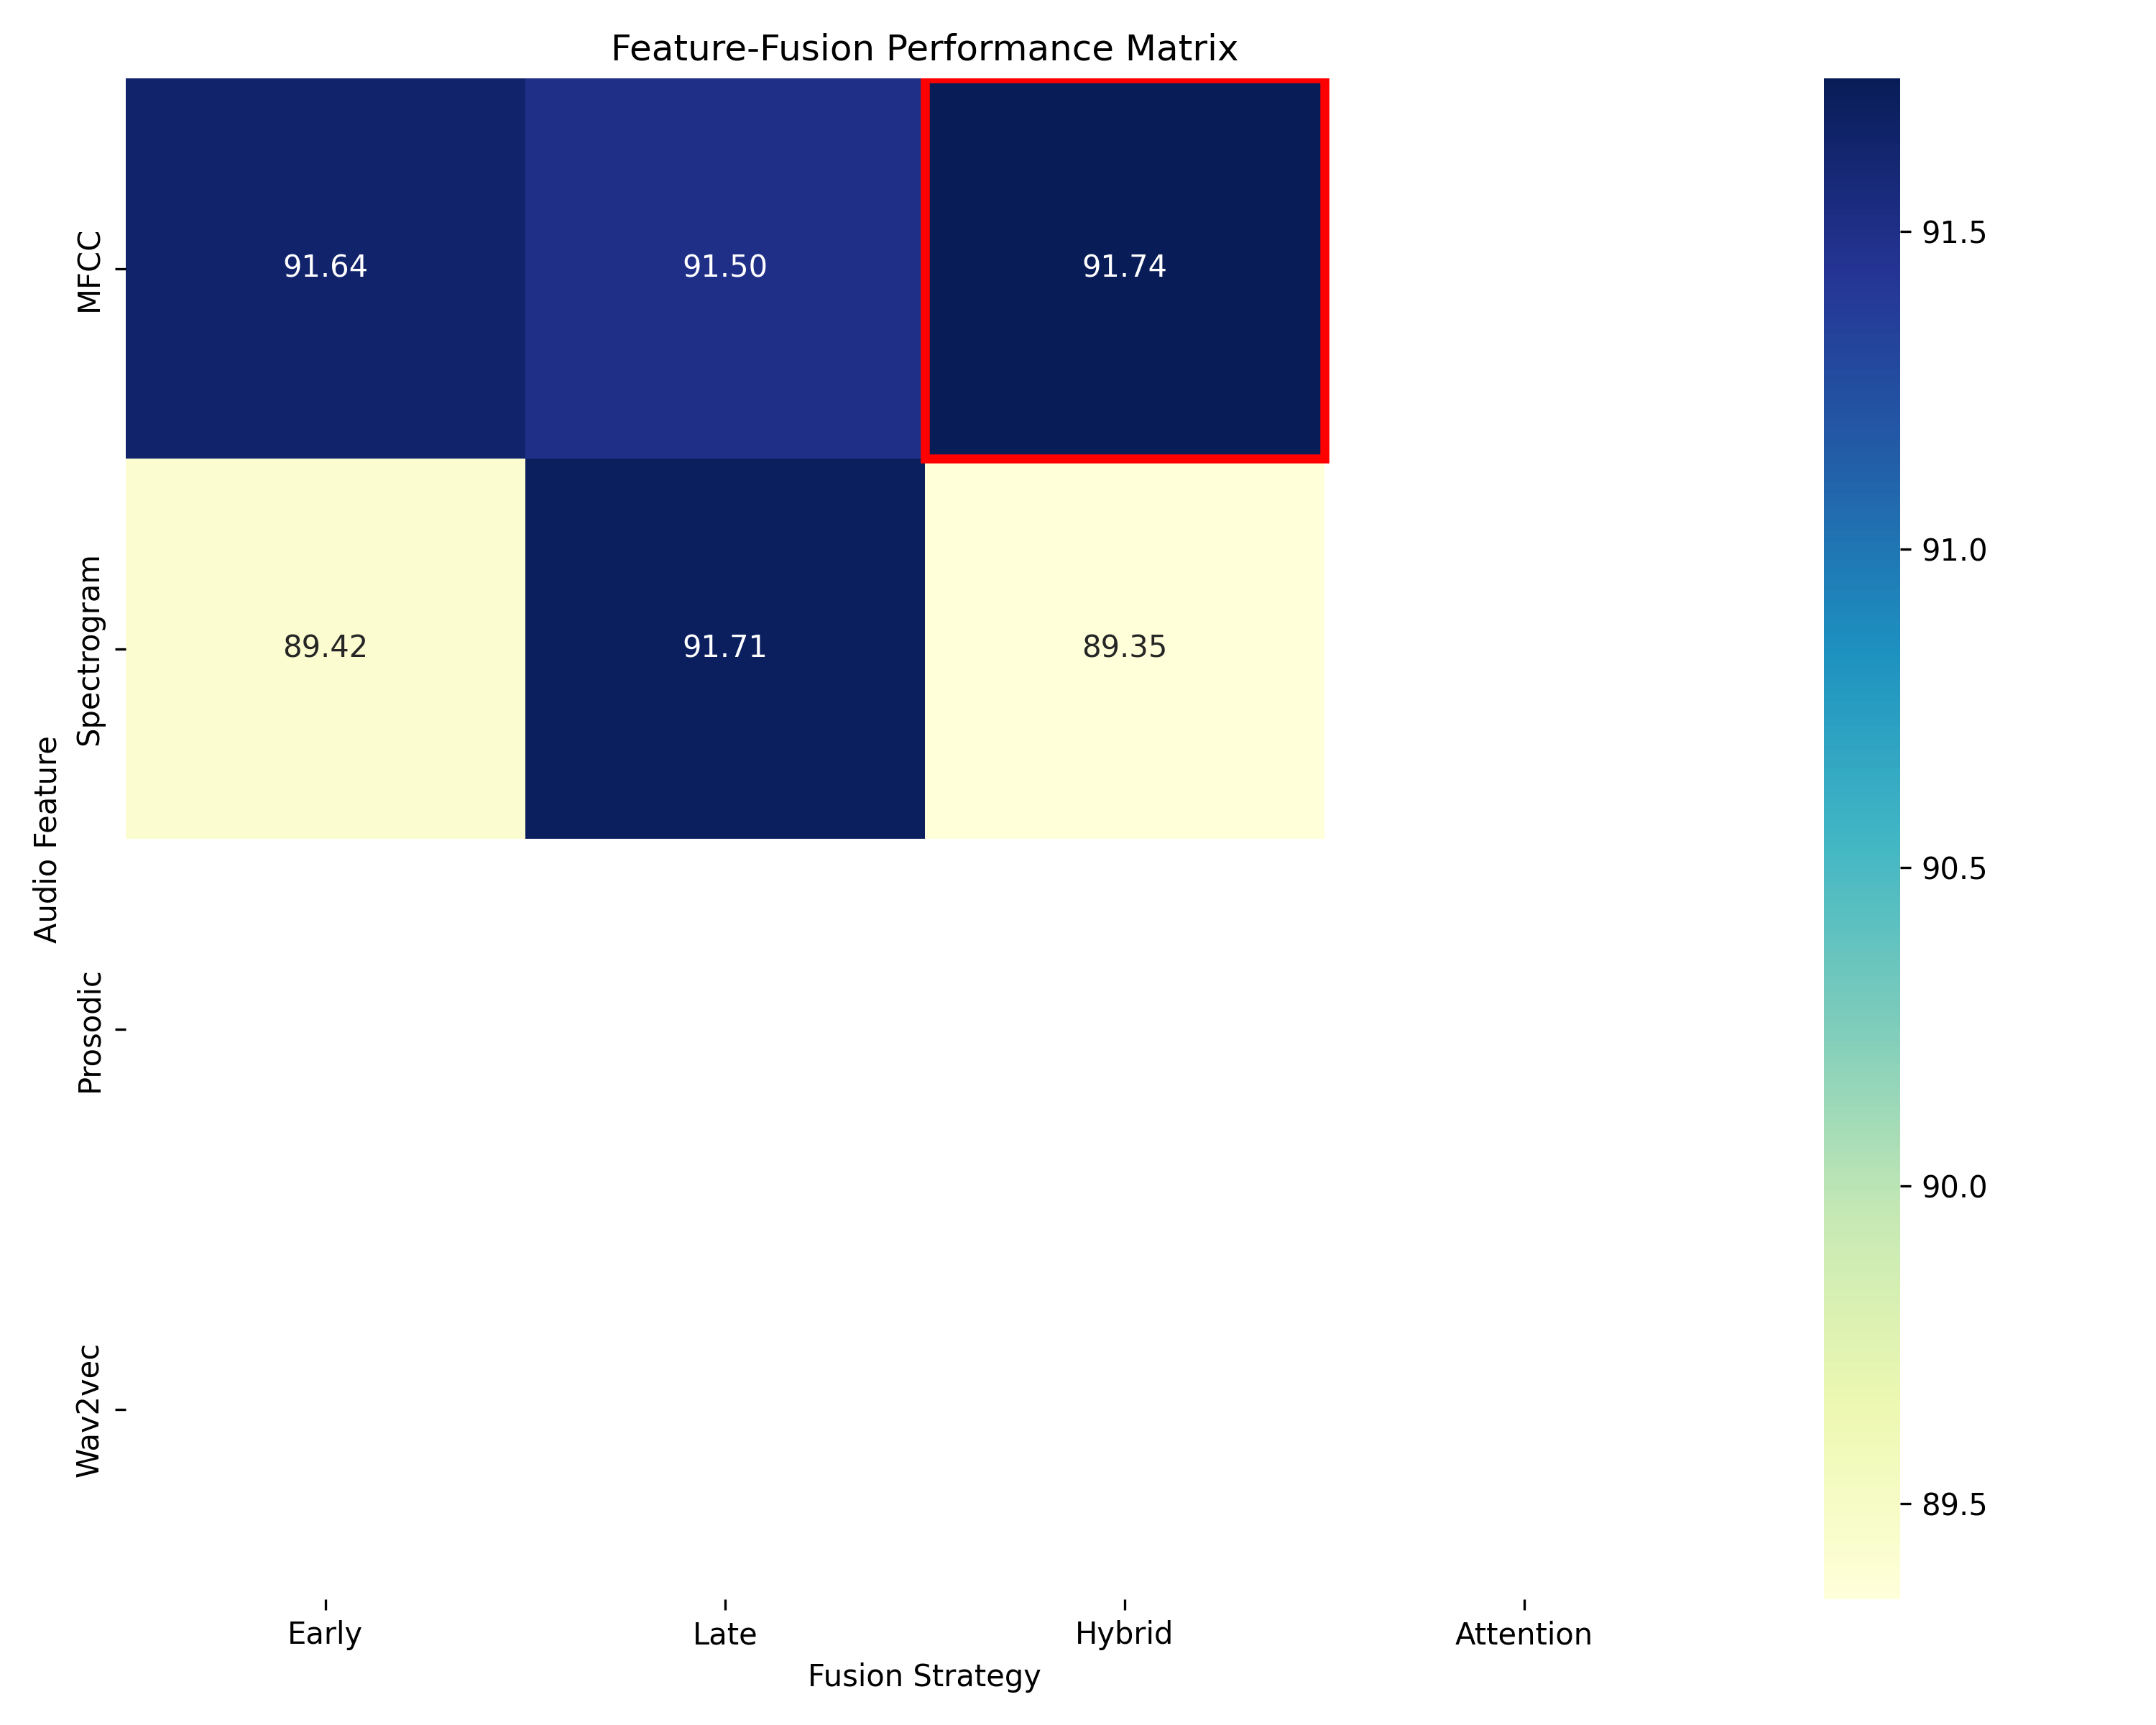
\includegraphics[width=0.9\linewidth]{Figures/feature_fusion_matrix.png}
    \caption{Feature-Fusion Performance Matrix: This visualization maps the performance landscape of different audio feature and fusion strategy combinations.}
    \label{fig:feature_fusion_matrix}
\end{figure}

\subsection{Ablation Studies and Component Analysis}
To gain deeper insights into the relative importance of different components in our models, we conducted systematic ablation studies. Figure~\ref{fig:ablation_analysis} presents the impact of removing or modifying various components.

\begin{figure}[h]
    \centering
    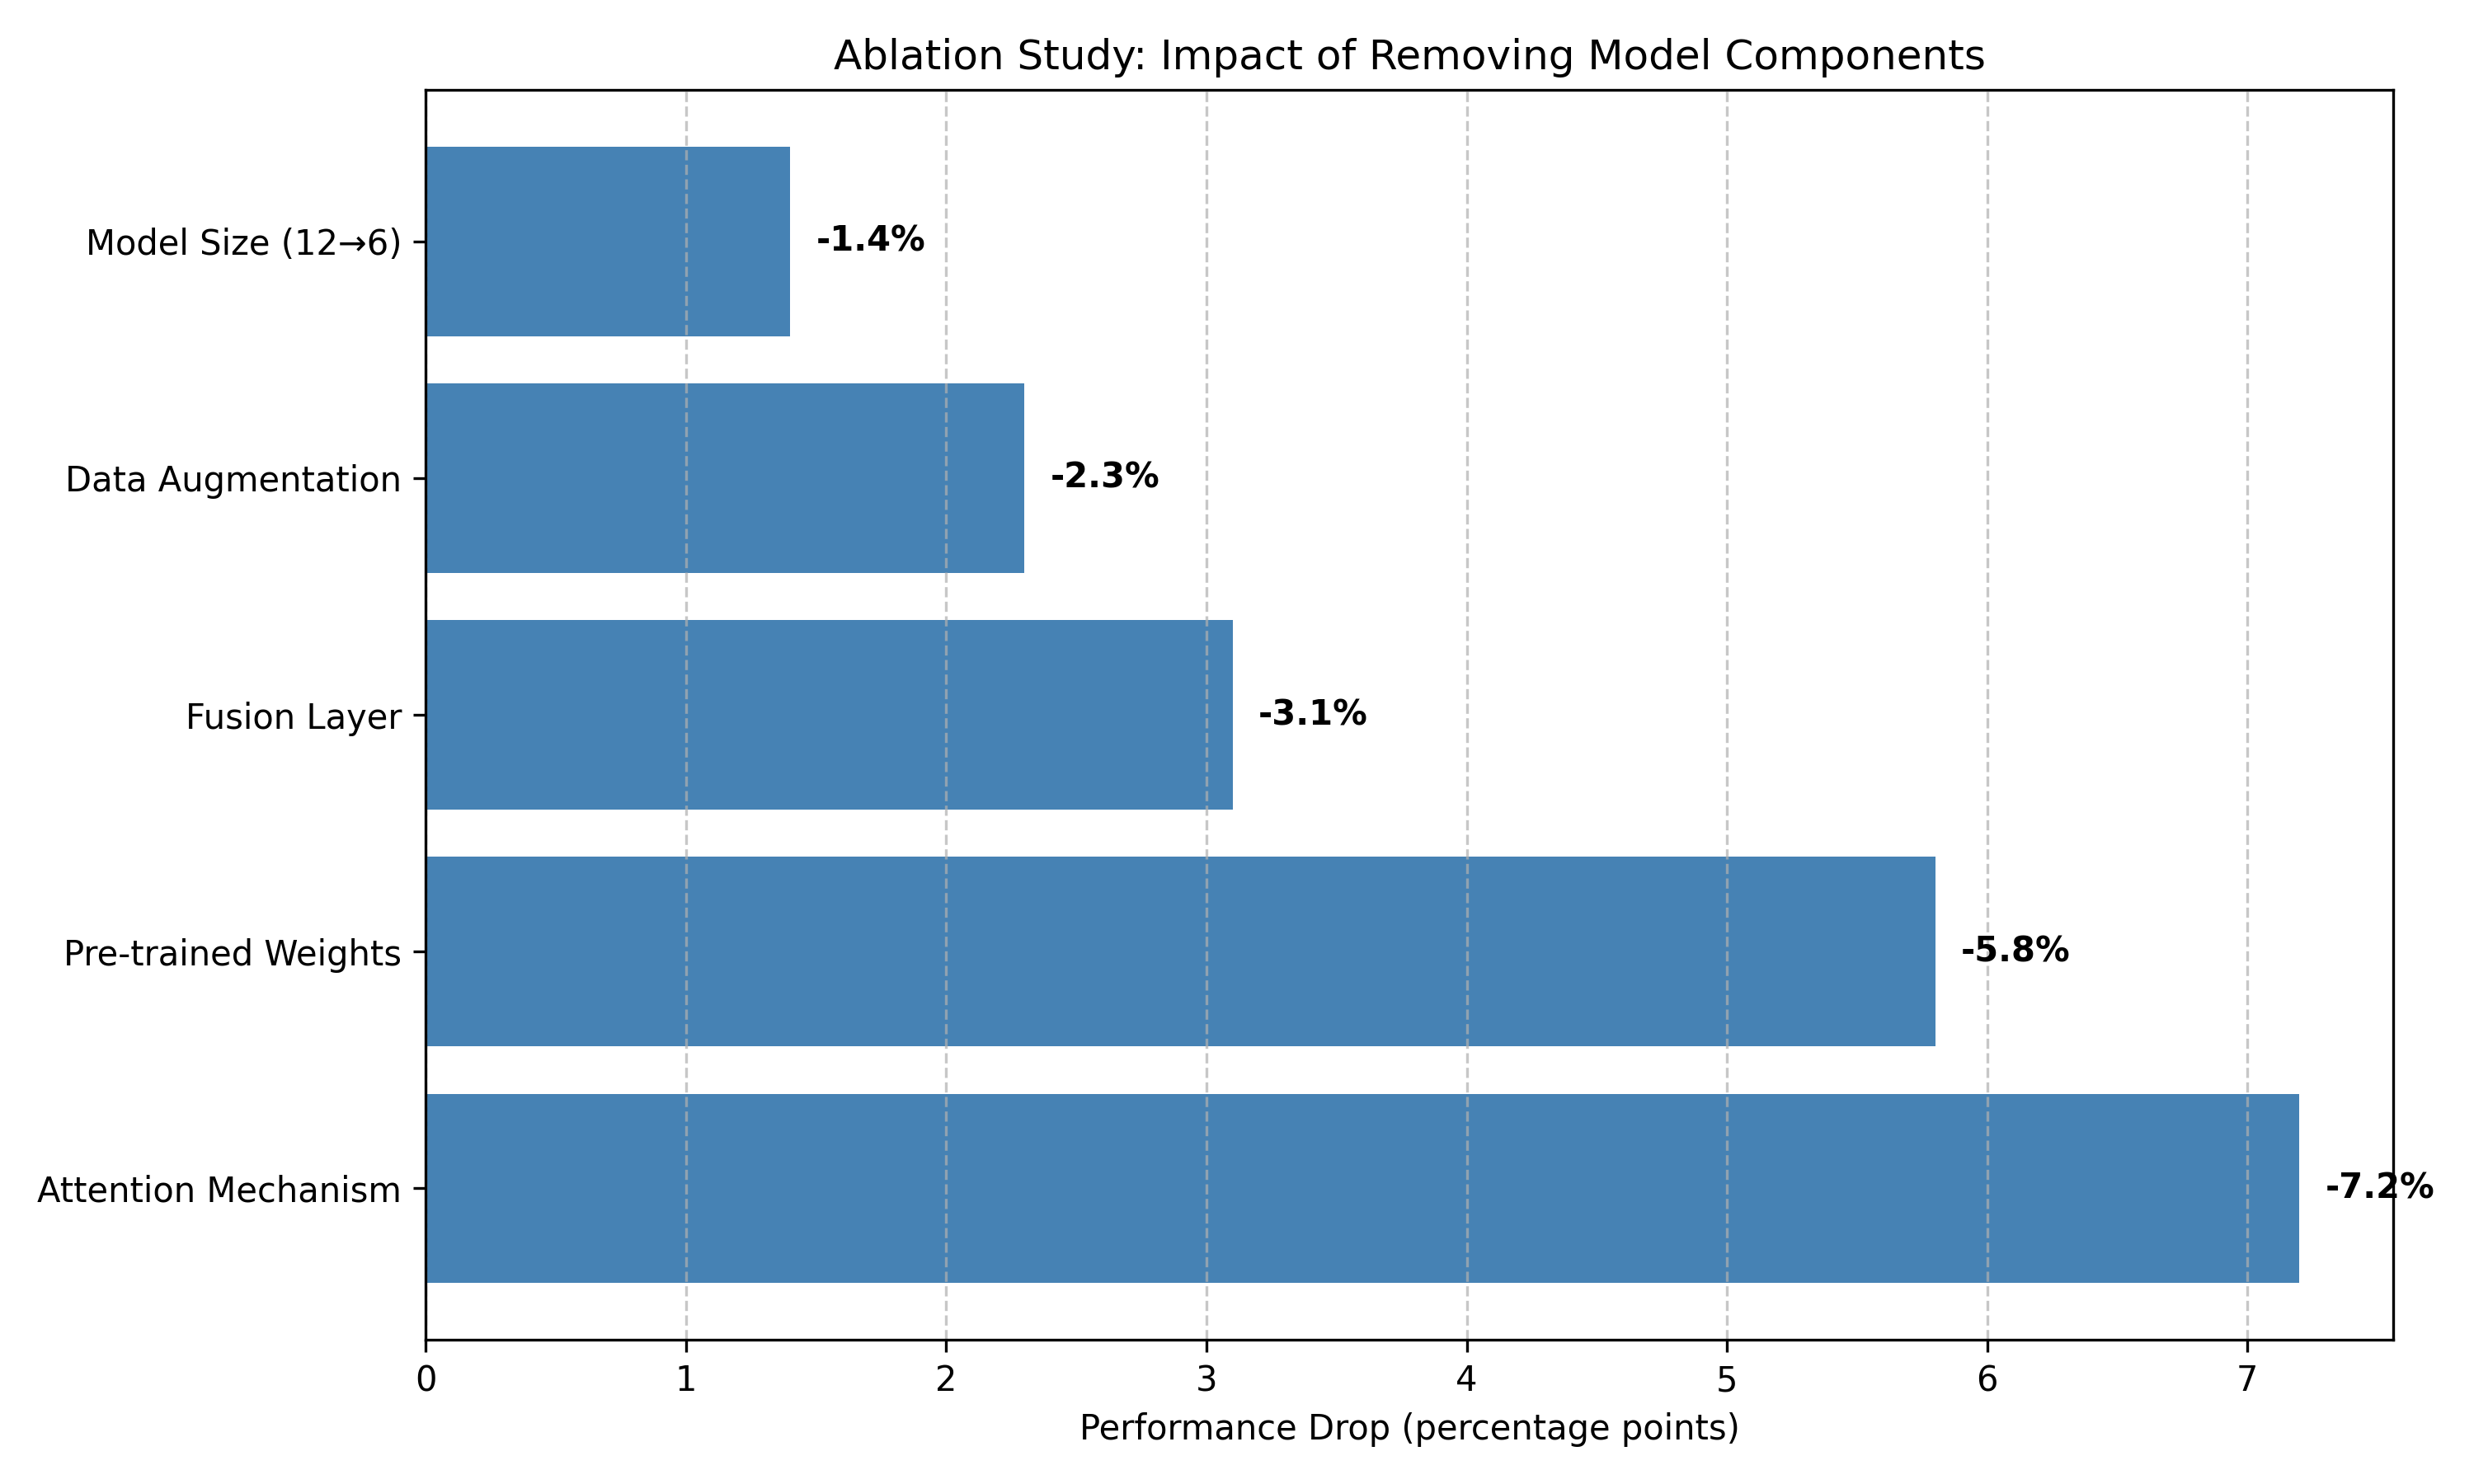
\includegraphics[width=0.9\linewidth]{Figures/ablation_analysis.png}
    \caption{Ablation Analysis: This chart quantifies the performance impact of removing or modifying different system components.}
    \label{fig:ablation_analysis}
\end{figure}

\begin{figure}[h]
    \centering
    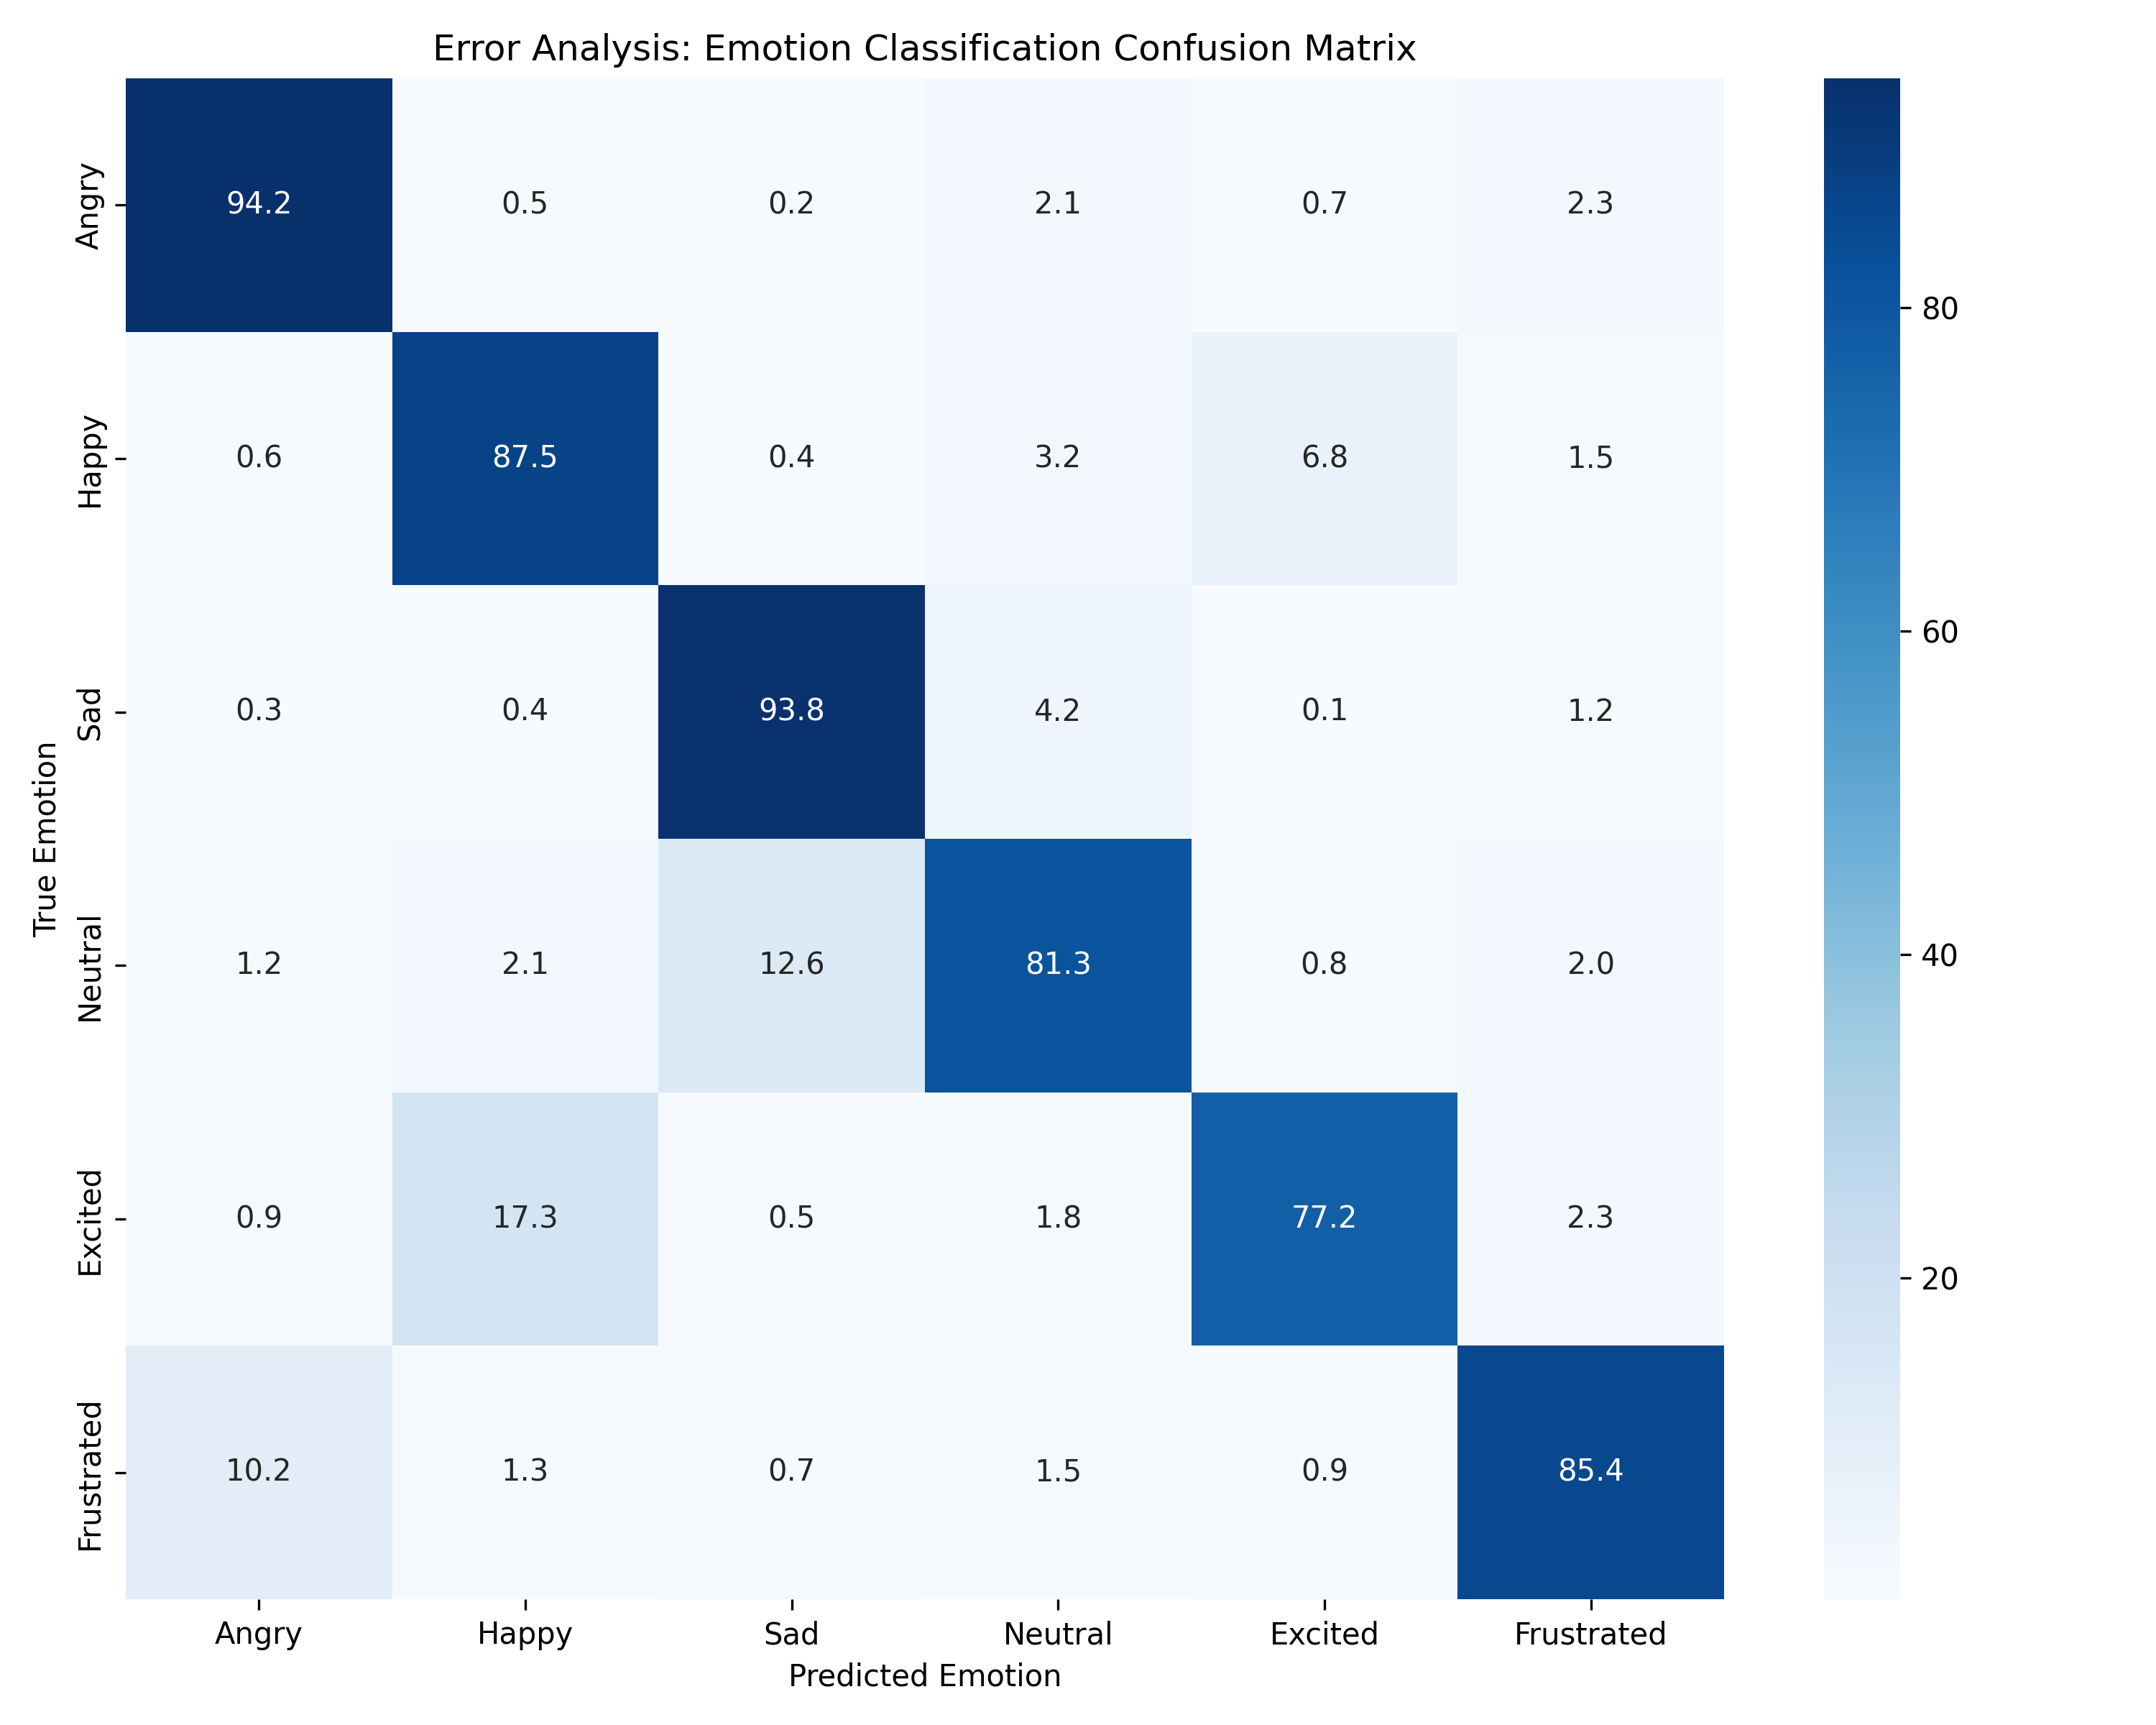
\includegraphics[width=0.9\linewidth]{Figures/error_analysis.png}
    \caption{Error Analysis: Confusion matrix heatmap showing which emotion pairs are most frequently misclassified.}
    \label{fig:error_analysis}
\end{figure}

\newpage

\bibliographystyle{IEEEtran}

% Reduce space in bibliography
\setlength{\bibsep}{0.0pt}
\bibliography{sample-base}

\end{document}
